%% abtex2-modelo-trabalho-academico.tex, v-1.9.7 laurocesar
%% Copyright 2012-2018 by abnTeX2 group at http://www.abntex.net.br/ 
%%
%% This work may be distributed and/or modified under the
%% conditions of the LaTeX Project Public License, either version 1.3
%% of this license or (at your option) any later version.
%% The latest version of this license is in
%%   http://www.latex-project.org/lppl.txt
%% and version 1.3 or later is part of all distributions of LaTeX
%% version 2005/12/01 or later.
%%
%% This work has the LPPL maintenance status `maintained'.
%% 
%% The Current Maintainer of this work is the abnTeX2 team, led
%% by Lauro César Araujo. Further information are available on 
%% http://www.abntex.net.br/
%%
%% This work consists of the files abntex2-modelo-trabalho-academico.tex,
%% abntex2-modelo-include-comandos and abntex2-modelo-references.bib
%%
% ------------------------------------------------------------------------
% ------------------------------------------------------------------------
% abnTeX2: Modelo de Trabalho Academico (tese de doutorado, dissertacao de
% mestrado e trabalhos monograficos em geral) em conformidade com 
% ABNT NBR 14724:2011: Informacao e documentacao - Trabalhos academicos -
% Apresentacao
% ------------------------------------------------------------------------
% ------------------------------------------------------------------------
%%
%% Documento ajustado para PCS-EPUSP em 15/mar/2023 por Cintia Borges Margi
% ------------------------------------------------------------------------
%%
\documentclass[
	% -- opções da classe memoir --
	12pt,				% tamanho da fonte
	openright,			% capítulos começam em pág ímpar (insere página vazia caso preciso)
	oneside,			% para impressão em recto e verso. Oposto a oneside
	a4paper,			% tamanho do papel. 
	% -- opções da classe abntex2 --
	%chapter=TITLE,		% títulos de capítulos convertidos em letras maiúsculas
	%section=TITLE,		% títulos de seções convertidos em letras maiúsculas
	%subsection=TITLE,	% títulos de subseções convertidos em letras maiúsculas
	%subsubsection=TITLE,% títulos de subsubseções convertidos em letras maiúsculas
	% -- opções do pacote babel --
	english,			% idioma adicional para hifenização
	french,				% idioma adicional para hifenização
	spanish,			% idioma adicional para hifenização
	brazil				% o último idioma é o principal do documento
	]{abntex2}

% ---
% Pacotes básicos 
% ---
\usepackage{lmodern}			% Usa a fonte Latin Modern			
\usepackage[T1]{fontenc}		% Selecao de codigos de fonte.
\usepackage[utf8]{inputenc}		% Codificacao do documento (conversão automática dos acentos)
\usepackage{indentfirst}		% Indenta o primeiro parágrafo de cada seção.
\usepackage{color}				% Controle das cores
\usepackage{graphicx}			% Inclusão de gráficos
\usepackage{microtype} 			% para melhorias de justificação
\usepackage{amsmath}
\usepackage{amssymb}
\usepackage{float}
\usepackage{subcaption}
\usepackage{tikz}
\usepackage{tikz-3dplot}
%\usetikzlibrary{arrows.meta} % for arrow size
\usetikzlibrary{3d} % for canvas is
\usepackage{circuitikz}
\usetikzlibrary{arrows,calc,positioning,fit}
\usetikzlibrary{angles,quotes} % for pic (angle labels)
\usetikzlibrary{arrows.meta}
\usetikzlibrary{backgrounds}
%\usepgfplotslibrary{patchplots}
%\usepgfplotslibrary{fillbetween}
\newcommand{\mixer}[2]
{  % #1 = reference coordinate, #2 = name
  \node[draw, thick, shape=circle, minimum size=24pt, at={#1}](#2){};
  \draw[rotate=45,line width=0.5pt] (#2.center)+(0,-12pt) -- +(0,12pt);
  \draw[rotate=-45,line width=0.5pt] (#2.center)+(0,-12pt) -- +(0,12pt);
}
\newcommand*{\vv}[1]{\vec{\mkern0mu#1}} % aligned vector arrow
\tikzstyle{axis}=[->,thick,line cap=round]
\newtheorem{theorem}{Theorem}

% ---
		
% ---
% Pacotes adicionais, usados apenas no âmbito do Modelo Canônico do abnteX2
% ---
\usepackage{lipsum}				% para geração de dummy text
% ---

% ---
% Pacotes de citações
% ---
\usepackage[brazilian,hyperpageref]{backref}	 % Paginas com as citações na bibl
\usepackage[alf]{abntex2cite}	% Citações padrão ABNT

%% CBM: pacote para incluir a ficha catalográfica como pdf
\usepackage[final]{pdfpages}

% --- 
% CONFIGURAÇÕES DE PACOTES
% --- 

% ---
% Configurações do pacote backref
% Usado sem a opção hyperpageref de backref
\renewcommand{\backrefpagesname}{Citado na(s) página(s):~}
% Texto padrão antes do número das páginas
\renewcommand{\backref}{}
% Define os textos da citação
\renewcommand*{\backrefalt}[4]{
	\ifcase #1 %
		Nenhuma citação no texto.%
	\or
		Citado na página #2.%
	\else
		Citado #1 vezes nas páginas #2.%
	\fi}%
% ---

% ---
% Informações de dados para CAPA e FOLHA DE ROSTO
% ---
\titulo{Modelo para TCC usando \abnTeX}
\autor{Aluno ...}
\local{São Paulo, SP}
\data{2023}
\orientador{Prof. Dr. Fulano}
\coorientador{Alguém?}
\instituicao{%
  Universidade de São Paulo -- USP
  \par
  Escola Politécnica
  \par
  Departamento de Engenharia de Computação e Sistemas Digitais (PCS)}
\tipotrabalho{Monografia de Conclusão de curso (Graduação)}
% O preambulo deve conter o tipo do trabalho, o objetivo, 
% o nome da instituição e a área de concentração 
\preambulo{Trabalho de conclusão de curso apresentado ao Departamento de Engenharia de Computação e Sistemas Digitais da Escola Politécnica da Universidade de São Paulo para obtenção do Título de Engenheiro.}
% ---


% ---
% Configurações de aparência do PDF final

% alterando o aspecto da cor azul
\definecolor{blue}{RGB}{41,5,195}

% informações do PDF
\makeatletter
\hypersetup{
     	%pagebackref=true,
		pdftitle={\@title}, 
		pdfauthor={\@author},
    	pdfsubject={\imprimirpreambulo},
	    pdfcreator={LaTeX with abnTeX2},
		pdfkeywords={abnt}{latex}{abntex}{abntex2}{trabalho acadêmico}, 
		colorlinks=true,       		% false: boxed links; true: colored links
    	linkcolor=blue,          	% color of internal links
    	citecolor=blue,        		% color of links to bibliography
    	filecolor=magenta,      		% color of file links
		urlcolor=blue,
		bookmarksdepth=4
}
\makeatother
% --- 

% ---
% Posiciona figuras e tabelas no topo da página quando adicionadas sozinhas
% em um página em branco. Ver https://github.com/abntex/abntex2/issues/170
\makeatletter
\setlength{\@fptop}{5pt} % Set distance from top of page to first float
\makeatother
% ---

% ---
% Possibilita criação de Quadros e Lista de quadros.
% Ver https://github.com/abntex/abntex2/issues/176
%
% \newcommand{\quadroname}{Quadro}
% \newcommand{\listofquadrosname}{Lista de quadros}

% \newfloat[chapter]{quadro}{loq}{\quadroname}
% \newlistof{listofquadros}{loq}{\listofquadrosname}
% \newlistentry{quadro}{loq}{0}

% % configurações para atender às regras da ABNT
% \setfloatadjustment{quadro}{\centering}
% \counterwithout{quadro}{chapter}
% \renewcommand{\cftquadroname}{\quadroname\space} 
% \renewcommand*{\cftquadroaftersnum}{\hfill--\hfill}

% \setfloatlocations{quadro}{hbtp} % Ver https://github.com/abntex/abntex2/issues/176
% ---

% --- 
% Espaçamentos entre linhas e parágrafos 
% --- 

% O tamanho do parágrafo é dado por:
\setlength{\parindent}{1.3cm}

% Controle do espaçamento entre um parágrafo e outro:
\setlength{\parskip}{0.2cm}  % tente também \onelineskip

% ---
% compila o indice
% ---
\makeindex
% ---

% ----
% Início do documento
% ----
\begin{document}

% Seleciona o idioma do documento (conforme pacotes do babel)
%\selectlanguage{english}
\selectlanguage{brazil}

% Retira espaço extra obsoleto entre as frases.
\frenchspacing 

% ----------------------------------------------------------
% ELEMENTOS PRÉ-TEXTUAIS
% ----------------------------------------------------------
% \pretextual

% ---
% Capa
% ---
\imprimircapa
% ---

% ---
% Folha de rosto
% (o * indica que haverá a ficha bibliográfica)
% ---
\imprimirfolhaderosto*
% ---

% ---
% Inserir a ficha bibliografica
% ---

% Isto é um exemplo de Ficha Catalográfica, ou ``Dados internacionais de
% catalogação-na-publicação''. Você pode utilizar este modelo como referência. 
% Porém, provavelmente a biblioteca da sua universidade lhe fornecerá um PDF
% com a ficha catalográfica definitiva após a defesa do trabalho. Quando estiver
% com o documento, salve-o como PDF no diretório do seu projeto e substitua todo
% o conteúdo de implementação deste arquivo pelo comando abaixo:
%
%% TODO: utilizar a ficha catalográfica gerada em https://www.poli.usp.br/bibliotecas/servicos/catalogacao-na-publicacao
\begin{fichacatalografica}
    \includepdf{ficha.pdf}
\end{fichacatalografica}

% \begin{fichacatalografica}
% 	\sffamily
% 	\vspace*{\fill}					% Posição vertical
% 	\begin{center}					% Minipage Centralizado
% 	\fbox{\begin{minipage}[c][8cm]{13.5cm}		% Largura
% 	\small
% 	\imprimirautor
% 	%Sobrenome, Nome do autor
	
% 	\hspace{0.5cm} \imprimirtitulo  / \imprimirautor. --
% 	\imprimirlocal, \imprimirdata-
	
% 	\hspace{0.5cm} \thelastpage p. : il. (algumas color.) ; 30 cm.\\
	
% 	\hspace{0.5cm} \imprimirorientadorRotulo~\imprimirorientador\\
	
% 	\hspace{0.5cm}
% 	\parbox[t]{\textwidth}{\imprimirtipotrabalho~--~\imprimirinstituicao,
% 	\imprimirdata.}\\
	
% 	\hspace{0.5cm}
% 		1. Palavra-chave1.
% 		2. Palavra-chave2.
% 		3. Palavra-chave3.
% 		I. Orientador.
% 		II. Universidade xxx.
% 		III. Faculdade de xxx.
% 		IV. Título 			
% 	\end{minipage}}
% 	\end{center}
% \end{fichacatalografica}
% ---

% ---
% Inserir errata
% ---
% \begin{errata}
% Elemento opcional da \citeonline[4.2.1.2]{NBR14724:2011}. Exemplo:

% \vspace{\onelineskip}

% FERRIGNO, C. R. A. \textbf{Tratamento de neoplasias ósseas apendiculares com
% reimplantação de enxerto ósseo autólogo autoclavado associado ao plasma
% rico em plaquetas}: estudo crítico na cirurgia de preservação de membro em
% cães. 2011. 128 f. Tese (Livre-Docência) - Faculdade de Medicina Veterinária e
% Zootecnia, Universidade de São Paulo, São Paulo, 2011.

% \begin{table}[htb]
% \center
% \footnotesize
% \begin{tabular}{|p{1.4cm}|p{1cm}|p{3cm}|p{3cm}|}
%   \hline
%    \textbf{Folha} & \textbf{Linha}  & \textbf{Onde se lê}  & \textbf{Leia-se}  \\
%     \hline
%     1 & 10 & auto-conclavo & autoconclavo\\
%    \hline
% \end{tabular}
% \end{table}

% \end{errata}
% ---

% ---
% Inserir folha de aprovação
% ---

% Isto é um exemplo de Folha de aprovação, elemento obrigatório da NBR
% 14724/2011 (seção 4.2.1.3). Você pode utilizar este modelo até a aprovação
% do trabalho. Após isso, substitua todo o conteúdo deste arquivo por uma
% imagem da página assinada pela banca com o comando abaixo:
%
% \begin{folhadeaprovacao}
% \includepdf{folhadeaprovacao_final.pdf}
% \end{folhadeaprovacao}
%
% \begin{folhadeaprovacao}

%   \begin{center}
%     {\ABNTEXchapterfont\large\imprimirautor}

%     \vspace*{\fill}\vspace*{\fill}
%     \begin{center}
%       \ABNTEXchapterfont\bfseries\Large\imprimirtitulo
%     \end{center}
%     \vspace*{\fill}
    
%     \hspace{.45\textwidth}
%     \begin{minipage}{.5\textwidth}
%         \imprimirpreambulo
%     \end{minipage}%
%     \vspace*{\fill}
%    \end{center}
        
%    Trabalho aprovado. \imprimirlocal, 24 de novembro de 2012:

%    \assinatura{\textbf{\imprimirorientador} \\ Orientador} 
%    \assinatura{\textbf{Professor} \\ Convidado 1}
%    \assinatura{\textbf{Professor} \\ Convidado 2}
%    %\assinatura{\textbf{Professor} \\ Convidado 3}
%    %\assinatura{\textbf{Professor} \\ Convidado 4}
      
%    \begin{center}
%     \vspace*{0.5cm}
%     {\large\imprimirlocal}
%     \par
%     {\large\imprimirdata}
%     \vspace*{1cm}
%   \end{center}
  
% \end{folhadeaprovacao}
% ---

% ---
% Dedicatória
% ---
\begin{dedicatoria}
   \vspace*{\fill}
   \centering
   \noindent
   \textit{Este trabalho é dedicado às crianças adultas que,\\
   quando pequenas, sonharam em se tornar cientistas.} \vspace*{\fill}
\end{dedicatoria}
% ---

% ---
% Agradecimentos
% ---
\begin{agradecimentos}
Os agradecimentos principais são direcionados ...

\end{agradecimentos}
% ---

% ---
% Epígrafe
% ---
% \begin{epigrafe}
%     \vspace*{\fill}
% 	\begin{flushright}
% 		\textit{...}
% 	\end{flushright}
% \end{epigrafe}
% ---

% ---
% RESUMOS
% ---

% resumo em português
\setlength{\absparsep}{18pt} % ajusta o espaçamento dos parágrafos do resumo
\begin{resumo}
 O resumo deve ressaltar o  objetivo, o método, os resultados e as conclusões do documento. 
 Deve ser escrito em parágrafo única, e tipicamente é menor do que uma página.(\ldots) 
 As palavras-chave devem figurar logo abaixo do resumo, antecedidas da expressão Palavras-chave:, separadas entre si por ponto e finalizadas também por ponto.

 \textbf{Palavras-chave}: latex. abntex. editoração de texto.
\end{resumo}

% resumo em inglês
\begin{resumo}[Abstract]
 \begin{otherlanguage*}{english}
   This is the english abstract.

   \vspace{\onelineskip}
 
   \noindent 
   \textbf{Keywords}: latex. abntex. text editoration.
 \end{otherlanguage*}
\end{resumo}

% % resumo em francês 
% \begin{resumo}[Résumé]
%  \begin{otherlanguage*}{french}
%     Il s'agit d'un résumé en français.
 
%    \textbf{Mots-clés}: latex. abntex. publication de textes.
%  \end{otherlanguage*}
% \end{resumo}

% % resumo em espanhol
% \begin{resumo}[Resumen]
%  \begin{otherlanguage*}{spanish}
%    Este es el resumen en español.
  
%    \textbf{Palabras clave}: latex. abntex. publicación de textos.
%  \end{otherlanguage*}
% \end{resumo}
% ---

% ---
% inserir lista de ilustrações
% ---
\pdfbookmark[0]{\listfigurename}{lof}
\listoffigures*
\cleardoublepage
% ---

% ---
% inserir lista de quadros
% ---
% \pdfbookmark[0]{\listofquadrosname}{loq}
% \listofquadros*
% \cleardoublepage
% ---

% ---
% inserir lista de tabelas
% ---
\pdfbookmark[0]{\listtablename}{lot}
\listoftables*
\cleardoublepage
% ---

% ---
% inserir lista de abreviaturas e siglas
% ---
\begin{siglas}
  \item[ABNT] Associação Brasileira de Normas Técnicas
  \item[abnTeX] ABsurdas Normas para TeX
\end{siglas}
% ---

% ---
% inserir lista de símbolos
% ---
\begin{simbolos}
  \item[$ \Gamma $] Letra grega Gama
  \item[$ \Lambda $] Lambda
  \item[$ \zeta $] Letra grega minúscula zeta
  \item[$ \in $] Pertence
\end{simbolos}
% ---

% ---
% inserir o sumario
% ---
\pdfbookmark[0]{\contentsname}{toc}
\tableofcontents*
\cleardoublepage
% ---


% ----------------------------------------------------------
% ELEMENTOS TEXTUAIS
% ----------------------------------------------------------
\textual

% Capítulo 1. Introdução
\chapter{Introduction}

An important application of filters is, given a noisy signal as input, to extract the best estimate of the desired information \cite{haykin_adaptive_1996}. 
When we know the correlation between the desired signal and noise, we can design fixed parameter filters to do the job. Among the fixed parameter filters, the 
Wiener Filter \cite{haykin_adaptive_1996,sayed_adaptive_2008,manolakis_statistical_2005} has a special space because it is an optimum estimator in the sense of 
mean-square error. When we do not know the correlation between the signal and noise or when we are working on a non-stationary environment, we can use an adaptive 
filter.

Adaptive filters are used in many problems, such as channel equalization, active noise reduction, series prediction, and system identification \cite{haykin_adaptive_1996,sayed_adaptive_2008,manolakis_statistical_2005}.
 Many types of adaptive filters are known, such as the Recursive-Least-Squares (RLS) filter, the Affine Projections filter, and the Least-Mean-Square (LMS) filter 
 \cite{haykin_adaptive_1996,sayed_adaptive_2008,manolakis_statistical_2005}. The latter uses the gradient descent algorithm to minimize the error between the output of 
 the filter and the desired signal. Its equations, which must be calculated for each sample, are
\begin{align}
    y(n) &= \mathbf{w}^{\top}(n-1)\mathbf{x}(n),\\
    e(n) &= d(n) - y(n),\\
    \mathbf{w}(n) &= \mathbf{w}(n-1) + \mu e(n)\mathbf{x}(n),
\end{align}
where $y(n)$ is the filter output, $\mathbf{w}(n)$ is a vector with the filter coefficients, $\mathbf{x}(n)$ is the filter input signal, $d(n)$ is the desired signal and $e(n)$ is 
the error. The parameter $\mu$ is known as the adaptation step and must be chosen so that the adaptation period and the mean-square error are adequate to the problem 
in question.

Nonlinear forms of adaptive filters have appeared in the literature. These filters can deal with the same problems as their linear counterparts, but can deal with nonlinearities. 
For example, in the case of nonlinear active noise reduction, the nonlinearities introduced by the amplifier and loudspeaker might need to be suppressed by the filter. To do 
that, the filter must have nonlinear parts to be adapted, which increases its complexity. Several ways of introducing nonlinearities have been suggested. 
Nonlinear adaptive filters based on Volterra series, which have the advantage of preserving linearity in the parameters, have been proposed \cite{taiho_koh_second-order_1985}, but these filters have the disadvantage of having too many coefficients.
Splines were used in \cite{scarpiniti_nonlinear_2013} to create a filter with a linear part and a nonlinear part, made of a spline, whose control points are adapted. This filter has few coefficients to be adapted, but the optimization needed is nonconvex.
Kernel Adaptive Filters (KAF) \cite{principe_kernel_2010} use the theory of Reproducing Kernel Hilbert Spaces and Positive Definite Kernels to deal with nonlinearities, and lead to good performance but require dictionaries and strategies to restrict their memory usage to a finite size.

This paper proposes the use of a fixed dictionary, based on a Cartesian grid for KAFs. The fixed dictionary has several advantages, most notably a fixed complexity and smaller memory requirements. In the remainder of this section we explain in more detail the advantages of the proposed algorithm, after some preliminary definitions.

\section{Reproducing Kernel Hilbert Spaces}

A function $\kappa(.,.), \mathcal{X}\times\mathcal{X}\rightarrow\mathbb{R}$ where $\mathcal{X} \subset \mathbb{R}^M$ is called a Positive Definite Kernel if, for any 
finite set of elements $\{\mathbf{x}_1,\mathbf{x}_2\,\dots,\mathbf{x}_n\} \in \mathcal{X}$, the matrices whose entries are $(\kappa(\mathbf{x}_i,\mathbf{x}_j))$, 
$i,j = \{1,2,\dots,n\}$, are nonnegative definite. It may be confusing to use the term Positive Definite Kernel when it creates nonnegative definite matrices, but this 
is the usual definition \cite{paulsen_introduction_2016}.

One form of characterizing a function as a Positive Definite Kernel is via Bochner's theorem \cite{wendland_scattered_2005}, which states that if a function $f(.), \mathbb{R}^M\rightarrow\mathbb{R}$ 
has a nonnegative Fourier transform, then $f(.-.)$ is a Positive Definite Kernel and the converse is also true, that is, if we have a nonnegative definite matrix with 
entries $f(\mathbf{x}_i-\mathbf{x}_j)$, then $f(.)$ must have a nonnegative Fourier transform.

A Reproducing Kernel Hilbert Space $\mathcal{H}$ (RKHS) is a Hilbert Space (a complete inner product space) of functions on $\mathcal{X} \subset \mathbb{R}^M$ with an 
evaluation functional $E_{\mathbf{x}},\mathcal{H} \rightarrow \mathbb{R}$ defined as $E_{\mathbf{x}}(f) = f(\mathbf{x})$. The Riesz representation theorem \cite{riesz_functional_2009} states that every 
linear functional on a Hilbert space can be represented as an inner product with an unique vector in $\mathcal{H}$, and so is the case of the evaluation functional. 
This way, the evaluation functional can be written as $E_{\mathbf{x}}(f) = \langle \kappa(\mathbf{x},.),f(.) \rangle_\mathcal{H} = f(\mathbf{x})$, where the function $\kappa(\mathbf{x},.)$ 
is known as the reproducing kernel for the point $\mathbf{x} \in \mathcal{X}$. The function $\kappa(.,.)$ is known as the reproducing kernel of $\mathcal{H}$ and the property
$\langle \kappa(\mathbf{x},.),f(.) \rangle_\mathcal{H} = f(\mathbf{x})$ is known as the reproducing property of the kernel $\kappa(.,.)$ \cite{paulsen_introduction_2016}. 

It is possible to show \cite{paulsen_introduction_2016} that if $\kappa(.,.)$ is the kernel of an RKHS, then $\kappa(.,.)$ is a Positive Definite Kernel. Also, if $\kappa(.,.)$ 
is a Positive Definite Kernel, we can show that there is a RKHS whose reproducing kernel is $\kappa(.,.)$ \cite{paulsen_introduction_2016}. We also use the fact that the 
set 
\begin{equation}
    \mathcal{H}_{\kappa} = \operatorname{span}\{\kappa(\mathbf{x},.), \forall \mathbf{x}\in \mathbb{R}^M\},
\end{equation}
is dense in $\mathcal{H}$ \cite{aronszajn_theory_1950}.

\section{Kernel Adaptive Filters}

Kernel methods \cite{scholkopf_learning_2002} use the theory of Positive Definite Kernels to transform a linear method based on inner products into a nonlinear one. 
To achieve this, the input vectors $\mathbf{x}_i$ are mapped to functions that belong to the RKHS as in
\begin{equation}
    \mathbf{x}_i \rightarrow \kappa(\mathbf{x}_i,.),
\end{equation}
and the inner products are calculated using these functions and the reproducing property of the kernel
\begin{equation}
    \langle \kappa(\mathbf{x}_i,.), \kappa(\mathbf{x}_j,.) \rangle_{\mathcal{H}} = \kappa(\mathbf{x}_i, \mathbf{x}_j).
\end{equation}

The use of kernels to create adaptive filters started with a version of the KRLS \cite{engel_kernel_2004} and then the Kernel-Least-Mean-Square (KLMS) \cite{liu_kernel_2008}, 
which gives the foundations of our work. As proposed in \cite{liu_kernel_2008}, the KLMS is defined by the following equations\footnote{By \eqref{eq:klms_w} we mean that $\mathbf{w}(n-1)$ is a function which applied to a vector $\mathbf{x}(n)$ results in $y(n)$ as in \eqref{eq:klms_y}}
\begin{align}
    \mathbf{w}(n-1) &= \sum_{i=1}^{n-1}\mu e(i)\kappa(\mathbf{x}(i),.)\label{eq:klms_w}\\
    y(n) &= \sum_{i=1}^{n-1}\mu e(i)\kappa(\mathbf{x}(i),\mathbf{x}(n))\label{eq:klms_y}\\
    e(n) &= d(n) - y(n)\\
    \mathbf{w}(n) &= \mathbf{w}(n-1) +\mu e(n)\kappa(\mathbf{x}(n),.).
\end{align}
We notice from these equations that the number of evaluations of kernel functions increases with $n$, which makes this filter impractical if used for many iterations. 
To avoid this memory growth, sparsification of dictionaries techniques were introduced.

\section{Sparsification of Dictionaries}

In these techniques, we create a set of input vectors with some distinctive characteristics known as a dictionary $\mathcal{D}$. Since we do not put every input vector 
in the dictionary, we expect fewer evaluations of the kernel function compared with the KLMS with no sparsification of dictionary. The first of these techniques proposed 
was the Novelty Criterion \cite{platt_resource-allocating_1991}. In the Novelty Criterion, we include an input vector in the dictionary if
\begin{equation}
    \min_{\mathbf{r}_i \in \mathcal{D}} ||\mathbf{x}(n) - \mathbf{r}_i||>\varepsilon_{NC},
\end{equation}
where $\varepsilon_{NC}$ is a chosen parameter. The Coherence Criterion \cite{richard_online_2009}, in turn, uses
\begin{equation}
    \min_{\mathbf{r}_i \in \mathcal{D}} \kappa(\mathbf{r}_i,\mathbf{x}(n)) < \varepsilon_{CC},
\end{equation}
where $\varepsilon_{CC}$ is again a chosen parameter. Quantized KLMS (QKLMS) \cite{badong_chen_quantized_2012} uses the same criterion as the Novelty Criterion to put 
vectors in the dictionary, but adapts the filter weight relative to the closest vector in the dictionary when the input vector is not included. Random Fourier Features (RFF-KLMS) \cite{bouboulis_efficient_2016} uses an 
approximation of the kernel using the theory of random Fourier features. The Approximate Linear Dependence only includes a new input vector in the dictionary if the kernel 
mapped from this vector is not close to a linear combination of the kernels mapped by the vectors in the dictionary \cite{engel_kernel_2004}. The latter technique is closely related with the GS-KLMS (Gram-Schmidt KLMS) technique, discussed next.

\section{GS-KLMS}\label{sec:gsklms}

In the GS-KLMS \cite{bueno_gram-schmidt-based_2020}, the input vectors $\mathbf{x}(n) \in \mathcal{X} \subset \mathbb{R}^M$ are first mapped to a kernel function 
$\kappa(\mathbf{x}(n),.) \in \mathcal{H}$ and then this kernel is projected in a vector subspace $\mathcal{B}\subset \mathcal{H}$. This vector subspace 
$\mathcal{B}$ is spanned by an orthonormal basis $\mathbf{B} = \{\boldsymbol{\beta}_1, \;\; \boldsymbol{\beta}_2, \;\; \dots, \;\; \boldsymbol{\beta}_N\}$. The fact that 
$\mathbf{B}$ is an orthonormal basis makes the calculation of the projections easy, since the projection norm in each direction $\boldsymbol{\beta}_i$ can be calculated 
as the inner product between the kernel mapped by the input vector and $\boldsymbol{\beta}_i$. To obtain the set $\mathbf{B}$, we start with the input vectors that 
were put in the dictionary $\mathcal{D}$, map them to kernels as $\kappa(\mathbf{r}_i,.)$, and apply the Gram-Schmidt process \cite{meyer_matrix_2023}
\begin{align}
    \boldsymbol{\beta}_1 &= \frac{\kappa(\mathbf{r}_1,.)}{||\kappa(\mathbf{r}_1,.)||},\label{eq:beta_1}\\
    \boldsymbol{\gamma}_i &= \kappa(\mathbf{r}_i,.) - \sum_{j=1}^{i-1}\langle\kappa(\mathbf{r}_i,.),\boldsymbol{\beta}_j\rangle_{\mathcal{H}}\boldsymbol{\beta}_j.\label{eq:gamma_i}\\
    \boldsymbol{\beta}_i &= \frac{\boldsymbol{\gamma}_i}{||\boldsymbol{\gamma}_i||}, \label{eq:beta_i}
\end{align}
Iterating equations \eqref{eq:beta_1}, \eqref{eq:gamma_i} and \eqref{eq:beta_i}, we can show that every $\boldsymbol{\beta}_i$ is a linear combination of kernels $\kappa(\mathbf{r}_j,.)$, that is
\begin{equation}
    \boldsymbol{\beta}_i = \sum_{j=1}^{i} h_{ij}\kappa(\mathbf{r}_j,.).
\end{equation}
We can group the values $h_{ij}$ in a matrix $\mathbf{H}$.

To verify whether a vector must be put in the dictionary, we compare the kernel norm $||\kappa(\mathbf{x}(n),.)||$ and the norm $||\mathbf{p}_\mathcal{B}(n)||$, where $\mathbf{p}_\mathcal{B}(n)$ is the projection of $\kappa(\mathbf{x}(n),.)$ in the subspace $\mathcal{B}$. 
First, we notice that 
\begin{equation}
    \kappa(\mathbf{x}(n),.) = \mathbf{p}_{\mathcal{B}} + \mathbf{p}_{\mathcal{B}^{\perp}},
\end{equation}
where $\mathbf{p}_{\mathcal{B}^{\perp}}$ is the projection of $\kappa(\mathbf{x}(n),.)$ in the space orthogonal to $\mathcal{B}$, Then, we calculate the squared norm
\begin{equation}
    ||\kappa(\mathbf{x}(n),.)||^2 = ||\mathbf{p}_\mathcal{B}||^2 + ||\mathbf{p}_{\mathcal{B}^{\perp}}||^2,
\end{equation}
since $\mathbf{p}_{\mathcal{B}}$ and $\mathbf{p}_{\mathcal{B}^{\perp}}$ are orthogonal. Since we are using only normalized kernels in this work, we can say that $||\kappa(\mathbf{x}(n),.)||^2 = \kappa(\mathbf{x}(n),\mathbf{x}(n)) = 1$ and we have
\begin{equation}
    ||\mathbf{p}_\mathcal{B}||^2 = 1 - ||\mathbf{p}_{\mathcal{B}^{\perp}}||^2.
\end{equation}
If the norms $||\kappa(\mathbf{x}(n),.)||$ and $||\mathbf{p}_\mathcal{B}||$ are close enough, that is, if 
\begin{equation}
    ||\mathbf{p}_{\mathcal{B}^{\perp}}||^2 < \varepsilon,
\end{equation}
where $\varepsilon$ is a chosen parameter, which means that if
\begin{equation}
    ||\mathbf{p}_\mathcal{B}||^2 > 1 - \varepsilon^2,
\end{equation}
we do not put the input vector in the dictionary. But, if the norms are very different, that is
\begin{equation}
    ||\mathbf{p}_\mathcal{B}||^2 < 1 - \varepsilon^2,
\end{equation}
we give the input vector $\mathbf{x}(n)$ a new 
name $\mathbf{r}_i$, include it in the dictionary $\mathcal{D}$ and update the basis $\mathbf{B}$, adding a new vector $\boldsymbol{\beta}_i$ using \eqref{eq:beta_1}, \eqref{eq:gamma_i} and \eqref{eq:beta_i}.

\begin{figure}
    \centering
    \begin{subfigure}[b]{0.4\linewidth}
        \centering
        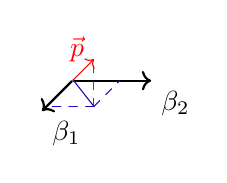
\begin{tikzpicture}
            \coordinate (O) at (0,0,0);
            \def\rvec{1.2}
            \def\thetavec{45}
            \def\phivec{45}
            \def\w{0.2}
            \tdplotsetcoord{O'}{0.04}{\thetavec}{\phivec} % shifted
            \tdplotsetcoord{O''}{0.1}{90}{\phivec} % shifted
            \tdplotsetcoord{P}{\rvec}{\thetavec}{\phivec}
            %\draw[axis] (0,0.02,0) -- (0,1,0) node[below right]{$z$};
            \draw[axis] (0,0,0.02) -- (0,0,1) node[below right]{$\beta_1$};
            \draw[axis] (0.02,0,0) -- (1,0,0) node[below right]{$\beta_2$};
            %\draw[->,red,line cap=round] (O'') -- (Pxy) node[anchor=130] {$\vv{p}_\mathrm{T}$};
            \draw[dashed,red,line join=round] (Pxz) -- (P);
            \draw[->,red,line cap=round] (O') -- (P) node[anchor=-30] {$\vv{p}$};
            \draw[-,blue,line cap=round] (Pxz) -- (O') node[anchor=-30] {};
            \draw[dashed,blue,line cap=round] (Pxz) -- (Px) node[anchor=-30] {};
            \draw[dashed,blue,line cap=round] (Pxz) -- (Pz) node[anchor=-30] {};
        \end{tikzpicture}
        \caption{inadequate}
    \end{subfigure}
    \begin{subfigure}[b]{0.4\linewidth}
        \centering
        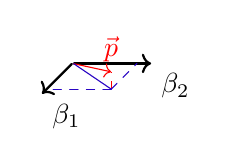
\begin{tikzpicture}
            \coordinate (O) at (0,0,0);
            \def\rvec{1.2}
            \def\thetavec{45}
            \def\phivec{15}
            \def\w{0.2}
            \tdplotsetcoord{O'}{0.04}{\thetavec}{\phivec} % shifted
            \tdplotsetcoord{O''}{0.1}{90}{\phivec} % shifted
            \tdplotsetcoord{P}{\rvec}{\thetavec}{\phivec}
            %\draw[axis] (0,0.02,0) -- (0,1,0) node[below right]{$z$};
            \draw[axis] (0,0,0.02) -- (0,0,1) node[below right]{$\beta_1$};
            \draw[axis] (0.02,0,0) -- (1,0,0) node[below right]{$\beta_2$};
            %\draw[->,red,line cap=round] (O'') -- (Pxy) node[anchor=130] {$\vv{p}_\mathrm{T}$};
            \draw[dashed,red,line join=round] (Pxz) -- (P);
            \draw[->,red,line cap=round] (O') -- (P) node[above] {$\vv{p}$};
            \draw[-,blue,line cap=round] (Pxz) -- (O') node[anchor=-30] {};
            \draw[dashed,blue,line cap=round] (Pxz) -- (Px) node[anchor=-30] {};
            \draw[dashed,blue,line cap=round] (Pxz) -- (Pz) node[anchor=-30] {};
        \end{tikzpicture}
        \caption{adequate}
    \end{subfigure} 
    \caption{Two possibilities of the projection}
    \label{fig:proj}
\end{figure}

We can create an adaptive filter using the projections $\mathbf{p}_{\mathcal{B}}(n)$, or, since it is easier, the vector of the coefficients of the projections 
\begin{align}
    \tilde{\mathbf{p}}_\mathcal{B}(n) &= \begin{bmatrix}
        \langle\kappa(\mathbf{x}(n),.),\boldsymbol{\beta}_1\rangle_\mathcal{H}\\
        \langle\kappa(\mathbf{x}(n),.),\boldsymbol{\beta}_2\rangle_\mathcal{H}\\
        \vdots\\
        \langle\kappa(\mathbf{x}(n),.),\boldsymbol{\beta}_N\rangle_\mathcal{H}\\
    \end{bmatrix} \\&= \begin{bmatrix}
        \langle\kappa(\mathbf{x}(n),.),\sum_{j=1}^{1}h_{1j}\kappa(\mathbf{r}_j,.)\rangle_\mathcal{H}\\
        \langle\kappa(\mathbf{x}(n),.),\sum_{j=1}^{2}h_{2j}\kappa(\mathbf{r}_j,.)\rangle_\mathcal{H}\\
        \vdots\\
        \langle\kappa(\mathbf{x}(n),.),\sum_{j=1}^{N}h_{Nj}\kappa(\mathbf{r}_j,.)\rangle_\mathcal{H}\\
    \end{bmatrix},      
\end{align}
which can be calculated as
\begin{equation}
    \tilde{\mathbf{p}}_{\mathcal{B}}(n) =\mathbf{H}\boldsymbol{\kappa}(\mathbf{x}(n)),
\end{equation}
where the coefficients of $\mathbf{H}$ can be obtained from \eqref{eq:beta_1}, \eqref{eq:gamma_i} and \eqref{eq:beta_i} and the vector $\boldsymbol{\kappa}(\mathbf{x}(n))$ is
\begin{equation}
    \boldsymbol{\kappa}(\mathbf{x}(n)) = \begin{bmatrix}
        \kappa(\mathbf{x}(n),\mathbf{r}_1)\\
        \kappa(\mathbf{x}(n),\mathbf{r}_2)\\
        \vdots\\
        \kappa(\mathbf{x}(n),\mathbf{r}_N)\\
    \end{bmatrix}.      
\end{equation}
The adaptive filter can then be calculated as
\begin{align}
    y(n) &= \mathbf{w}^{\top}(n-1)\tilde{\mathbf{p}}_{\mathcal{B}}(n)\\
    e(n) &= d(n) - y(n)\\
    \mathbf{w}(n) &= \mathbf{w}(n-1) + \mu e(n)\tilde{\mathbf{p}}_{\mathcal{B}}(n).
\end{align}

This algorithm works well, but still has a growing dictionary, which may lead to variable computational cost and steady-state performance.
In the following sections we propose a new kernel adaptive filtering algorithm with fixed complexity, based on a Cartesian grid dictionary.

\section{Structure of the work}
In Section \ref{sec:grids}, we present how Cartesian grids are generated, the kernels we are using in this work, and orthonormalization procedures. After that, techniques to
choose the parameters of the filters are presented in Section \ref{sec:choice}. Section \ref{sec:simulations} shows examples obtained with numerical simulations and the conclusions
are in Section \ref{sec:conclusions}


% Capítulo 2. Aspectos Conceituais
\chapter{Cartesian Grids of Kernel Functions and Orthonormalization}\label{sec:grids}

In this work, we use Cartesian grids as dictionaries for kernel least-mean-square filters. Cartesian grids are grids of points disposed in the space as the vertices of squares, cubes or hypercubes, whose edges are parallel to the system axes. 

\section{Cartesian Grids}

Usually, kernel filters use ad-hoc dictionaries \cite{engel_kernel_2004,richard_online_2009,platt_resource-allocating_1991,badong_chen_quantized_2012,bueno_gram-schmidt-based_2020}, that is, the dictionary is created as the input vectors arrive and in the order they arrive. This depends on the input vector distribution and may cause problems if outliers arrive, since outliers usually are put on the dictionary, causing more computation than should be needed. Also, even after orthonormalization, as in the case of the GS-KLMS, different realizations of the process that generates the input vectors could result in different dictionaries, and may even lead to the Mean Squared Error to have a different behavior. 
Figure \ref{fig:err2_sparsifications} shows four the Mean Square Error of 10 realizations of a KLMS with different sparsification techniques (Novelty Criterion, Coherence Criterion, Gram-Schmidt and the Cartesian Grid proposed in this work). It is possible to see that the Cartesian Grid have smaller variation of the MSE in steady state between realisations.
%\textcolor{red}{Put figure showing the MSE for different realizations and with different sparsification methods.}
\begin{figure}
    \centering
    \begin{subfigure}[b]{0.45\linewidth}
        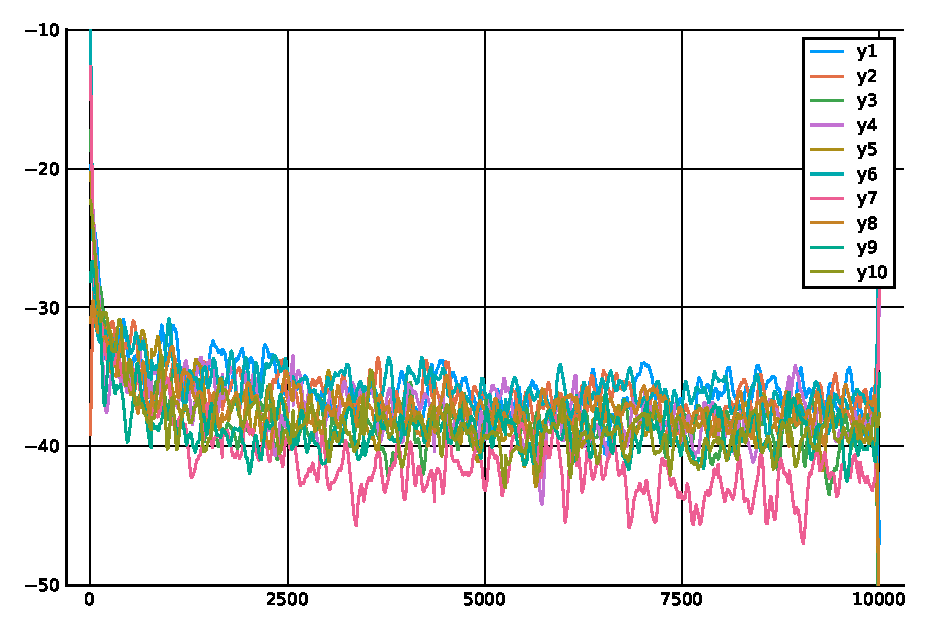
\includegraphics[width=\linewidth]{figuras/err2_nc_sparse.eps}
        \caption{}
        \label{fig:err2_nc}
    \end{subfigure}
    \begin{subfigure}[b]{0.45\linewidth}
        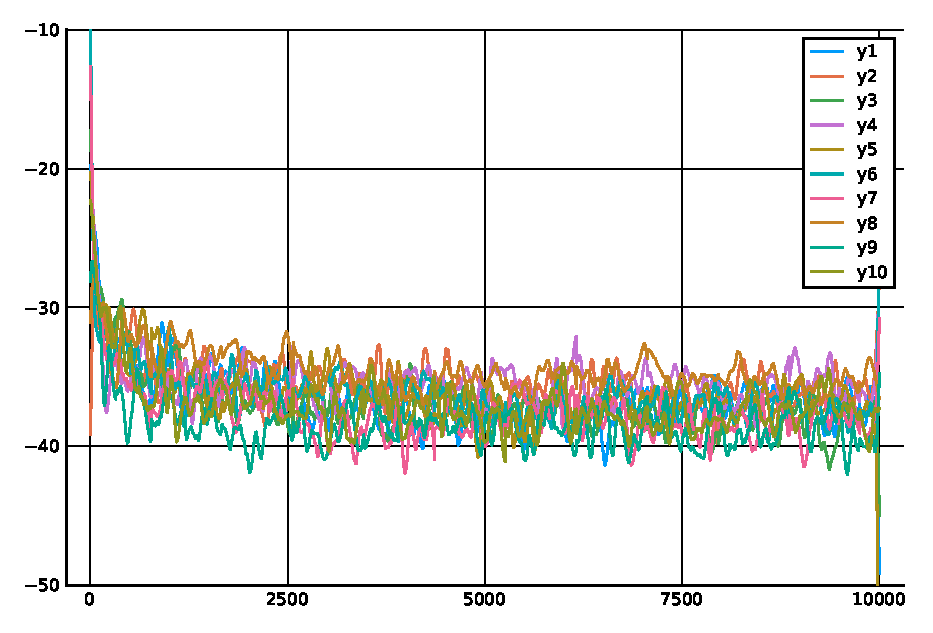
\includegraphics[width=\linewidth]{figuras/err2_cc_sparse.eps}
        \caption{}
        \label{fig:err2_cc}
    \end{subfigure}
    \begin{subfigure}[b]{0.45\linewidth}
        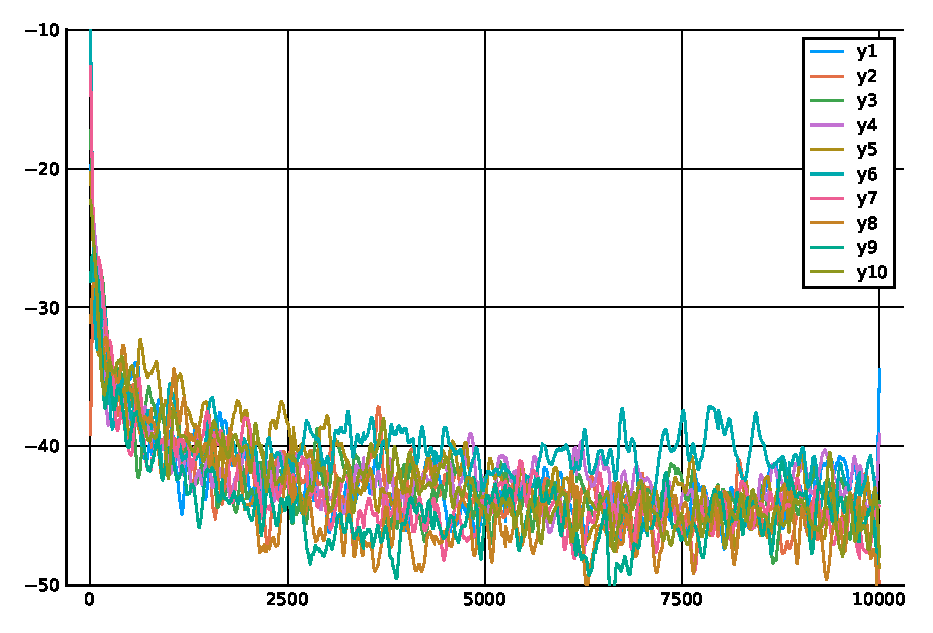
\includegraphics[width=\linewidth]{figuras/err2_gs_sparse.eps}
        \caption{}
        \label{fig:err2_gs}
    \end{subfigure}
    \begin{subfigure}[b]{0.45\linewidth}
        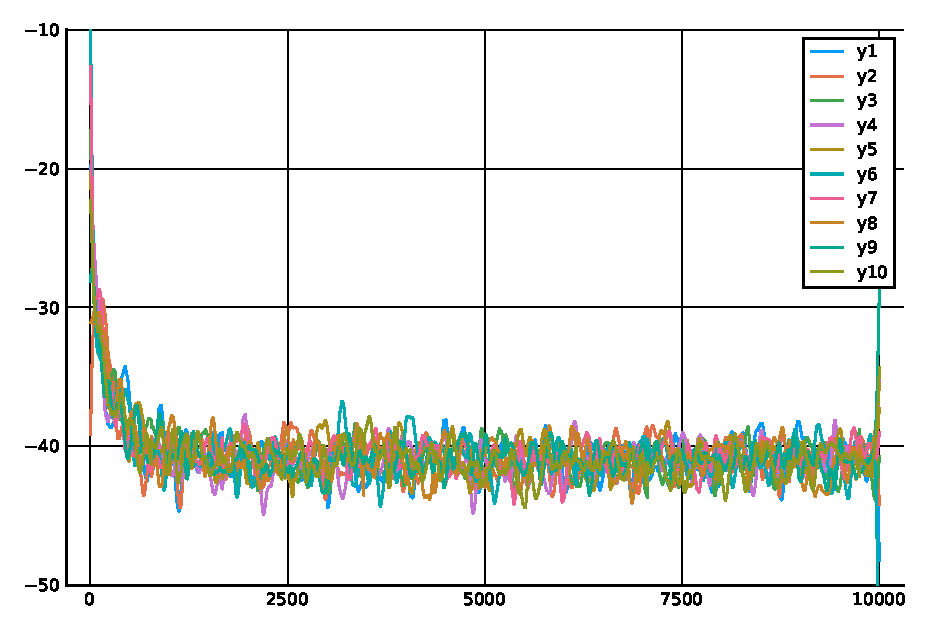
\includegraphics[width=\linewidth]{figuras/err2_cg_sparse.eps}
        \caption{}
        \label{fig:err2_cg}
    \end{subfigure}
    \caption{Mean Square Error for 10 evaluations of 4 different sparsification techniques: (a) Novelty Criterion; (b) Coherence Criterion; (c) Gram-Schmidt; (d) Cartesian Grid}
    \label{fig:err2_sparsifications}
\end{figure}

The grid dictionary we peopose here is chosen at design time, which result in different realizations of the input vectors process having similar MSE. Since the MSE of different realizations are similar, stochastic analysies will be more predictive. Cartesian grids \cite{thompson_handbook_1999} are a type of regular grid with their roots in the integer lattice $\mathbb{Z}^M$ \cite{conway_sphere_1993}. This is a simple grid when compared to others like rhombohedric, irregular grids or others based on different coordinate systems. A dictionary based on a Cartesian grid can be defined as the set
\begin{equation}
    \mathcal{D} = \{ \mathbf{r}_i = \rho\mathbf{z}_i\;|\;\rho \in \mathbb{R}, \mathbf{z}_i \in \mathbb{Z}^M \},\label{eq:grid}
\end{equation}
where $\rho$ is the grid parameter and is the only parameter needed to define it. This means that we have (only) one more parameter to choose in the design of the filter. The index $i$ is in the range $\{1, 2, \dots, N\} $ and the cardinality of the dictionary $|\mathcal{D}| = N$ depends on both the input set $\mathcal{X}$ and the grid parameter.

Some kernels and their parameters are better suited than others when using a Cartesian grid as a dictionary. Radial basis functions \cite{buhmann_radial_2003,scholkopf_learning_2002}, that depend on the distance between points, are good choices since we are choosing exactly the localization of these points. Other kernels with the form $f(.-.)$ are also good choices for the same reason.
% Kernels that depend on other factors, for example, polynomial kernels \cite{scholkopf_learning_2002} that depend on inner product of their variables, are not good choices since the evaluation of the kernel with two vectors that are close but orthogonal as arguments will have a low value.

\section{Kernel Functions and their characteristics}

Three kernel functions were chosen for this work because of their characteristics: 

\subsection{Gaussian Kernel}

The Gaussian kernel 
\begin{equation}
    \kappa(\mathbf{x},\mathbf{y}) = e^{-\frac{||\mathbf{x} - \mathbf{y}||^2}{2\sigma^2}}
\end{equation}
is the most used kernel in the literature of kernel adaptive filters \cite{principe_kernel_2010} because of its approximation properties. It is a normal kernel, which means that 
\begin{equation*}
  \kappa(\mathbf{x},\mathbf{x}) = 1, \forall \mathbf{x} \in \mathcal{X},  
\end{equation*}
and this is its maximum value. It is also a radial basis function, which means that
\begin{equation*}
    \kappa(\mathbf{x},\mathbf{y}) = \phi(||\mathbf{x} - \mathbf{y}||),
\end{equation*}
that is, it is a function of the distance between its arguments. 
We can see the gaussian kernel as the product of many functions, each in one dimension as
\begin{equation}
    e^{-\frac{||\mathbf{x} - \mathbf{y}||^2}{2\sigma^2}} = e^{-\frac{\sum_{i=1}^{M}(x_i-y_i)^2}{2\sigma^2}} = \prod_{i=1}^{M}e^{-\frac{(x_i-y_i)^2}{2\sigma^2}},
\end{equation}
which is known as a tensor product of functions \cite{boor_box_1993}.
The Gaussian kernel has the universal approximation characteristic \cite{steinwart_influence_2002}, which is proved using the Stone-Weierstrass theorem \cite{rudin_functional_2007}. 
% The Stone-Weierstrass theorem \cite{rudin_functional_2007} states that 
% \begin{theorem}
%     (Stone-Weierstrass theorem) Let $(\mathbf{X,d})$ be a compact metric space and $\mathbf{A}(\mathbf{X})$ an algebra of functions. Then $\mathbf{A}(\mathbf{X})$ is dense in $\mathbf{C}(\mathbf{X})$ (the set of continuous functions whose domain is $\mathbf{X}$) if
%     \begin{enumerate}
%         \item for all $x \in \mathbf{X}$, there is an  $f(.) \in \mathbf{A}(\mathbf{X})$ so that $f(x)\neq0$ and
%         \item for all $x,y \in \mathbf{X}$, with $x \neq y$, there is an $f(.)$ so that $f(x) \neq f(y)$.
%     \end{enumerate}
% \end{theorem}
Universal approximation is a characteristic of some sets of functions that, under certain conditions, are dense in another larger set, that is, given a member of the larger set, there is a member of the smaller set that is arbitrarily close to that member. The Stone-Weierstrass theorem guarantees that the set of linear combinations of gaussians is dense in the set of continuous functions.

Despite all of these good characteristics, the Gaussian kernel has a bad one: its support is equal to its domain. The support of a function whose domain is the set $\mathcal{X}$ is defined as \cite{rudin_functional_2007}
\begin{equation}
    \operatorname{supp}_{f(.)} = \{ \mathbf{x} \in \mathcal{X} | f(\mathbf{x}) \neq 0 \},
\end{equation}
but the Gaussian kernel is nowhere equal to zero. Because of this, when using the Gaussian kernel in a kernel adaptive filter, we need $N$ (the number of points in the dictionary) evaluations of the kernel function in each iteration. This means that the greater $N$, the greater the computational power needed. In the case of a dictionary on a Cartesian grid, this translates to the lower $\rho$ in \eqref{eq:grid}, the greater $N$ and so the larger the computational power.

\subsection{Tensor Product of Sincs}

% The Sinc function 
% \begin{equation}
%     \operatorname{sinc}(x) = \begin{cases}
%         \frac{\sin{\pi x}}{\pi x} \quad if \quad x \neq 0\\
%         1  \quad \;\; \quad if \quad x = 0
%     \end{cases}
% \end{equation}
% is well known in the field of signal processing because it is used in sampling theory \cite{oppenheim_discrete-time_2010}. When calculated as

% it is 
The reproducing kernel of an RKHS known as the Paley-Wiener space is given by
\begin{equation}
\kappa(x,y) = \operatorname{sinc}\left( \frac{x-y}{\sigma}\right),
\end{equation}
where the sinc function is
\begin{equation}
    \operatorname{sinc}(x) = \begin{cases}
        \frac{\sin{\pi x}}{\pi x} \quad \text{if} \quad x \neq 0;\\
        1  \quad \;\; \quad \text{if} \quad x = 0.
    \end{cases}
\end{equation}
The members of this space are band-limited functions with a known bandwidth. Sampling theory tells us that this function is capable of regenerating every band-limited function with adequate bandwidth, so that we can assume this to be a universal approximating characteristic for a class of functions.

Since it is a kernel, the product of many of these functions is also a kernel. That is
\begin{equation}
    \kappa(\mathbf{x},\mathbf{y}) = \prod_{i=1}^M \operatorname{sinc}\left( \frac{x_i-y_i}{\sigma} \right),
\end{equation}
is a multivariate kernel. This kernel is also normal, since $\operatorname{sinc}(0) = 1$ and its support is
\begin{equation}
    \operatorname{supp}_{\kappa(\mathbf{x},\mathbf{y})} = \left\{ \mathbf{x},\mathbf{y}\in \mathbb{R}^M \middle| \frac{x_i- y_i}{\sigma} \neq n, n \in \mathbb{Z}^* \right\}
\end{equation}
which means that it is unbounded.

The problem with the support of the Gaussian and tensor product of Sincs kernels motivates us to find another kernel with their desirable characteristics, i.e., normality and universal approximation characteristic, but with a compact support. A kernel with these characteristics is introduced in the next section.

\subsection{Tensor Product of B-Splines}

B-Splines are functions that have been used in interpolation and approximation of functions for decades now \cite{boor_box_1993}. The B-Spline is defined iteratively, starting with the B-Spline of order $0$
\begin{equation}
    b_0(x) = \begin{cases}
            0 \quad \text{if}  \quad x<-\frac{1}{2};\\
            1 \quad \text{if}  \quad -\frac{1}{2} \leq x \leq \frac{1}{2};\\
            0 \quad \text{if}  \quad x \geq \frac{1}{2}.
    \end{cases}
\end{equation}
The other orders are defined as
\begin{equation}
    b_{i+1}(x) = b_i(x)*b_0(x),
\end{equation}
where $*$ is the convolution operation. This means that the B-Spline of order $1$ is
\begin{equation}
    b_0(x) = \begin{cases}
            0 \quad \quad \;\;\; \text{if}  \quad x<-1;\\
            1+x \quad \text{if}  \quad -1 \leq x \leq 0;\\
            1-x \quad \text{if}  \quad 0 \leq x \leq 1;\\
            0 \quad \quad \;\;\; \text{if}  \quad x > 1.
    \end{cases}
\end{equation}
We can see that the support of the B-Spline of order $1$ is the open interval $(-1,1)$.
We can create a positive definite kernel as \cite{scholkopf_learning_2002}
\begin{equation*}
    \kappa(\mathbf{x},\mathbf{y}) = b_i\left( \frac{x-y}{\sigma}\right),
\end{equation*}
where $\sigma$ is its parameter.
A Tensor Product of B-Splines of order $1$ is defined as
\begin{equation}
    B_1(\mathbf{x}) = \prod_{i=1}^{M}b_1(x_i),
\end{equation}
which has a support in the set
\begin{equation*}
    \operatorname{supp}_{B_1(.)} = \underbrace{(-1,1)\times(-1,1)\times \dots\times(-1,1)}_{M \text{factors}}.
\end{equation*}
The Tensor Product of B-Splines of order $1$ kernel
\begin{equation*}
    \kappa(\mathbf{x},\mathbf{y}) = B_1\left( \frac{\mathbf{x} - \mathbf{y}}{\sigma} \right)
\end{equation*}
is a positive definite kernel since it is the multiplication of positive definite kernels \cite{aronszajn_theory_1950}.
It is easy to see that this kernel is of compact support and normal.

To show that this kernel has the universal approximation function, instead of the Stone-Weierstrass theorem, we use Wiener's Tauberian theorem. This theorem states that \cite{wiener_tauberian_1932}
\begin{theorem}
    (Wiener's Tauberian Theorem) Let $f(.) \in \mathcal{L}^2$ (the set of square integrable functions according to the Lebesgue integral) and $f(.+\lambda)$ be the class of translations of $f(.)$. If the Fourier transform of $f(.)$ has zeros that form a set of zero measure, then, given any $g(.) \in \mathcal{L}^2$ and any $\varepsilon_T > 0$, we have a set of coefficients $c_k$ and a set of translations $f(.+\lambda_k)$ such that $g_1(.) = \sum_k c_kf(.+\lambda_k)$ satisfies 
    \begin{equation*}
        \int_{\infty}^{\infty}|g(x) - g_1(x)|^2dx \leq \varepsilon_T.
    \end{equation*}
\end{theorem}

In this case, the set of kernels $\kappa(\mathbf{y},.), \;\; \mathbf{y}\in \mathbb{R}^M$ forms a dense subset of the set of square integrable functions over $\mathbf{X}$, $\mathcal{L}^2$, instead of the set of continuous functions as in the case of the Stone-Weierstrass theorem.

The Tensor product of B-Splines only needs sums and multiplications and no other functions like the exponential as needed to calculate the Gaussian kernel or the sine in sinc. This means that these functions can be easily calculated in an arithmetic logical unit in fixed point arithmetic, without the need for floating point operations, which is suitable for microcontrollers that do not have Floating Point Units.

\section{Orthonormalization procedures}

To create projections of the kernels mapped from the input vectors, we need to create an orthonormal basis from the set of kernels mapped from the vectors in the dictionary. The new basis vectors are linear combinations of the kernels mapped from the vectors of the dictionary
\begin{equation}
    \boldsymbol{\beta}_i = \sum_{j=1}^{M}h_{ij}\kappa(\mathbf{r}_j,.), \mathbf{r}_j \in \mathcal{D}.\label{eq:linearComb}
\end{equation}
We need to guarantee that the inner products of two $\boldsymbol{\beta}_i$, $i=1,2,\dots,N$, are given by
\begin{equation}
    \langle \boldsymbol{\beta}_i, \boldsymbol{\beta}_j \rangle_{\mathbf{B}} = \delta_{ij},\label{eq:KronDelta}
\end{equation}
where $\delta_{ij}$ is the usual Kronecker delta, that is, it is zero if $i \neq j$ and one if $i = j$.
Substituting \eqref{eq:linearComb} in \eqref{eq:KronDelta}, we have
\begin{equation}
    \langle \sum_{\ell=1}^{M}h_{i\ell}\kappa(\mathbf{r}_\ell,.), \sum_{m=1}^{M}h_{jm}\kappa(\mathbf{r}_m,.) \rangle_{\mathbf{B}} = \delta_{ij}.
\end{equation}
Using the linear properties of the inner product and the reproducing property of the kernel, we have
\begin{equation}
    \sum_{\ell=1}^{M}h_{i\ell}\sum_{m=1}^{M}h_{jm}\kappa(\mathbf{r}_\ell,\mathbf{r}_m) = \delta_{ij},
\end{equation}
which can be written in matrix form
\begin{equation}
    \mathbf{H} \mathbf{G} \mathbf{H}^{\top} = \mathbf{I},
\end{equation}
where matrix $\mathbf{G}$ is given by
\begin{equation}
    \mathbf{G} = \left[\begin{matrix}
        \kappa(\mathbf{r}_1,\mathbf{r}_1) & \kappa(\mathbf{r}_1,\mathbf{r}_2) & \dots & \kappa(\mathbf{r}_1,\mathbf{r}_N)\\
        \kappa(\mathbf{r}_2,\mathbf{r}_1) & \kappa(\mathbf{r}_2,\mathbf{r}_2) & \dots & \kappa(\mathbf{r}_2,\mathbf{r}_N)\\
        \vdots & \vdots & \ddots & \vdots\\
        \kappa(\mathbf{r}_N,\mathbf{r}_1) & \kappa(\mathbf{r}_N,\mathbf{r}_2) & \dots & \kappa(\mathbf{r}_N,\mathbf{r}_N)
    \end{matrix}\right],
\end{equation}
and is known as Grammian.
Multiplying by $\left(\mathbf{H}^{\top}\right)^{-1}\mathbf{G}^{-1}$ on the right, we get
\begin{equation}
    \mathbf{H} = \left(\mathbf{H}^{\top}\right)^{-1}\mathbf{G}^{-1},
\end{equation}
where $\left(\mathbf{H}^{\top}\right)^{-1}$ and $\mathbf{G}^{-1}$ exist since both $\{\kappa(\mathbf{r}_i,.)\}$ and $\{\boldsymbol{\beta}_i\}$ are linearly independent.
Multiplying by $\mathbf{H}^{\top}$ on the left, we arrive at
\begin{equation}
    \mathbf{H}^{\top}\mathbf{H} = \mathbf{G}^{-1},\label{eq:HtHG-1}
\end{equation}
so that any $\mathbf{H}$ that orthonormalizes the set of kernels that are mapped by the vectors of the dictionary must satisfy \eqref{eq:HtHG-1}.

One possible $\mathbf{H}$ is obtained using the Cholesky decomposition of $\mathbf{G}^{-1}$, and this corresponds to the Gram-Schmidt orthonormalization procedure since the matrix $\mathbf{H}^{GS}$ obtained in this decomposition is triangular and so one of the $\boldsymbol{\beta}_i$ depends only on one kernel, another of the $\boldsymbol{\beta}_i$ depends on two kernels, and so on.

A second possibility to satisfy \eqref{eq:HtHG-1} is to use 
\begin{equation}
    \mathbf{H}^{LS} = \mathbf{G}^{-\frac{1}{2}},
\end{equation}
where $\mathbf{G}^{-\frac{1}{2}}$ is calculated as
\begin{equation}
    \mathbf{G}^{-\frac{1}{2}} = \mathbf{V}\left[\begin{matrix}
        \frac{1}{\sqrt{\lambda_1}} & 0 & \dots & 0\\
        0 & \frac{1}{\sqrt{\lambda_2}} & \dots & 0\\
        \vdots & \vdots & \vdots & \vdots\\
        0 & 0 & \dots & \frac{1}{\sqrt{\lambda_M}}\\
    \end{matrix}\right]\mathbf{V}^{\top},
\end{equation}
with $\mathbf{V}$ the matrix whose columns are the eigenvectors of $\mathbf{G}$ and $\{\lambda_i\}$ its eigenvelues.
This choice is known in the Quantum Chemistry community as Löwdin Symmetric Orthonormalization \cite{mayer_lowdins_2002}. This procedure minimizes the sum of squared distances \cite{carlson_orthogonalization_1957}
\begin{equation}
    \sum_{i=1}^{M} ||\boldsymbol{\beta}_i - \kappa(\mathbf{r}_i,.)||^2.
\end{equation}

Since $\mathbf{H}^{GS}$ is obtained by the Cholesky factorization of $\mathbf{G}^{-1}$ and $\mathbf{H}^{LS}$ is obtained by calculating the squared root of $\mathbf{G}^{-1}$, we can say that $\mathbf{H}^{GS}$ is the triangular factor of the QR decomposition of $\mathbf{H}^{LS}$ \cite{horn_matrix_2017}.

\begin{figure}
    \centering
    \begin{subfigure}[b]{0.45\linewidth}
        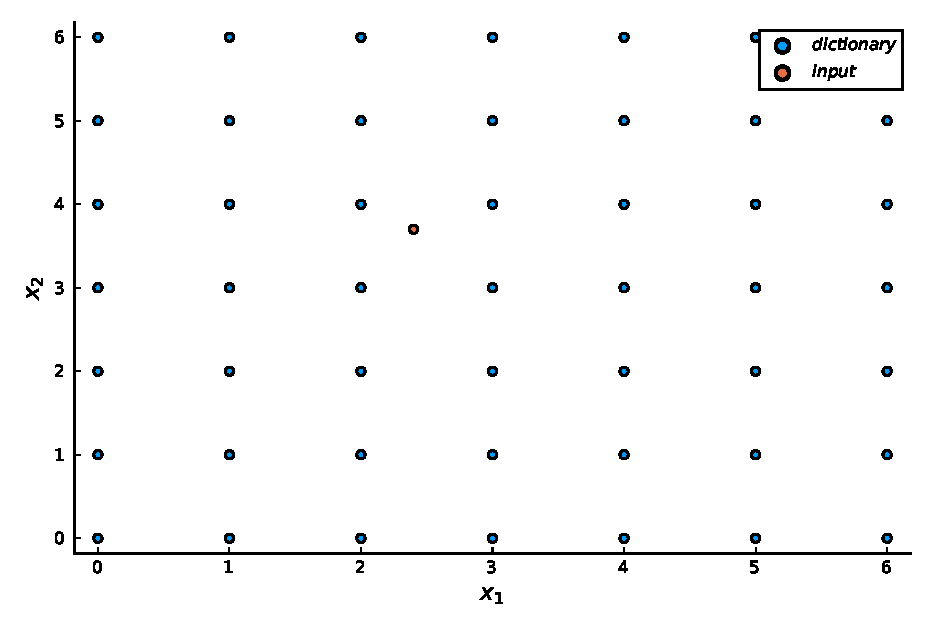
\includegraphics[width=\linewidth]{figuras/scatter_tpbs.eps}
        \caption{}
        \label{fig:tpbs_scatter_1}
    \end{subfigure}
    \begin{subfigure}[b]{0.45\linewidth}
        \includegraphics[width=\linewidth]{figuras/scatter_tpbs_05.eps}
        \caption{}
        \label{fig:tpbs_scatter_05}
    \end{subfigure}
    \caption{Dictionary points and input vector in a Cartesian grid}
    \label{fig:tpbs_scatter}
\end{figure}


Another useful characteristic of the tensor product of sincs and the tensor product of B-Splines of order $1$ is that if we use the parameter of the grid $\rho$ equal to the parameter of the kernel $\sigma$, the Gram matrix is already equal to the identity, meaning that they form an orthonormal basis \cite{horn_matrix_2017}. 
In the case of the tensor product of B-Splines, to compute the output of the filter, we only need to compute the kernels whose dictionary points are the vertices of the hypercube containing the input vector, and not the $N$ kernels mapped from the vectors of the dictionary, because the others are zero. This means that the computational cost (in terms of operations) of the filter is maintained if we use a lower $\rho$. On the other hand, since the number of vectors in the dictionary is bigger with a lower $\rho$, we need more memory to store the filter weights.
This is shown in Figure \ref{fig:tpbs_scatter}. The blue dots represent the dictionary points while the red dot represents the input vector, which is $(2.4,3.7)$. In the system of Figure \ref{fig:tpbs_scatter}\subref{fig:tpbs_scatter_1}, $\sigma = \rho = 1$. In this case, we don't need to compute the kernels corresponding to dictionary points with $x_1 < 1.4$ or $x_1 > 3.4$ since these will result in 0. The same is true for $x_2 < 2.7$ and $x_2 > 4.7$. This leaves us only the kernels corresponding to the points $\mathcal{V}_1 = \left\{(2,3),(3,3),(2,4),(3,4)\right\}$ which are the vertices of the square which contain the input vector.
In the case of the Figure \ref{fig:tpbs_scatter}\subref{fig:tpbs_scatter_05}, $\sigma = \rho = 0.5$, and, using the same reasoning, it is only needed to compute the kernels corresponding to points $\mathcal{V}_2 = \left\{(2,3.5),(2.5,3.5),(2.5,4),(2,4)\right\}$.


\subsection{Example with Gaussian kernels}

In this section, we show an example of orthonormalization of Gaussian kernels using Löwdin Symmetric and Gram-Schmidt techniques. We use nine Gaussian kernels with $\sigma = 1$ and 
centers at $C = \{(0,0),(1,0),(2,0),(0,1),(1,1),(2,1),(0,2),(1,2),(2,2)\}$. 

The matrices obtained for the Gram-Schmidt and for the Löwdin Symmetric techniques are in equations \eqref{eq:H_GS} and \eqref{eq:H_LS} respectively.

% \begin{figure}
%     \begin{subfigure}[b]{\linewidth}
        \begin{equation}
\resizebox{\linewidth}{!}{
$\mathbf{H}^{GS} = \left[
\begin{array}{ccccccccc}
1.0000 & 0.0000 & 0.0000 & 0.0000 & 0.0000 & 0.0000 & 0.0000 & 0.0000 & 0.0000 \\
-0.7629 & 1.2578 & 0.0000 & 0.0000 & 0.0000 & 0.0000 & 0.0000 & 0.0000 & 0.0000 \\
0.4976 & -1.1222 & 1.3526 & 0.0000 & 0.0000 & 0.0000 & 0.0000 & 0.0000 & 0.0000 \\
-0.7629 & -0.0000 & -0.0000 & 1.2578 & 0.0000 & 0.0000 & 0.0000 & 0.0000 & 0.0000 \\
0.5820 & -0.9595 & -0.0000 & -0.9595 & 1.5820 & 0.0000 & 0.0000 & 0.0000 & 0.0000 \\
-0.3796 & 0.8561 & -1.0319 & 0.6259 & -1.4115 & 1.7013 & 0.0000 & 0.0000 & 0.0000 \\
0.4976 & 0.0000 & -0.0000 & -1.1222 & -0.0000 & -0.0000 & 1.3526 & 0.0000 & 0.0000 \\
-0.3796 & 0.6259 & 0.0000 & 0.8561 & -1.4115 & -0.0000 & -1.0319 & 1.7013 & 0.0000 \\
0.2476 & -0.5584 & 0.6731 & -0.5584 & 1.2594 & -1.5179 & 0.6731 & -1.5179 & 1.8296 \\
\end{array}
\right]\label{eq:H_GS}$}
\end{equation}

%     \end{subfigure}    
% \end{figure}
% \begin{figure}
%     \begin{subfigure}[b]{\linewidth}
        \begin{equation}
\resizebox{\linewidth}{!}{
$\mathbf{H}^{LS} = \left[
\begin{array}{ccccccccc}
1.5324 & -0.6442 & 0.2011 & -0.6442 & 0.2708 & -0.0846 & 0.2011 & -0.0846 & 0.0264 \\
-0.6442 & 1.8772 & -0.6442 & 0.2708 & -0.7892 & 0.2708 & -0.0846 & 0.2464 & -0.0846 \\
0.2011 & -0.6442 & 1.5324 & -0.0846 & 0.2708 & -0.6442 & 0.0264 & -0.0846 & 0.2011 \\
-0.6442 & 0.2708 & -0.0846 & 1.8772 & -0.7892 & 0.2464 & -0.6442 & 0.2708 & -0.0846 \\
0.2708 & -0.7892 & 0.2708 & -0.7892 & 2.2997 & -0.7892 & 0.2708 & -0.7892 & 0.2708 \\
-0.0846 & 0.2708 & -0.6442 & 0.2464 & -0.7892 & 1.8772 & -0.0846 & 0.2708 & -0.6442 \\
0.2011 & -0.0846 & 0.0264 & -0.6442 & 0.2708 & -0.0846 & 1.5324 & -0.6442 & 0.2011 \\
-0.0846 & 0.2464 & -0.0846 & 0.2708 & -0.7892 & 0.2708 & -0.6442 & 1.8772 & -0.6442 \\
0.0264 & -0.0846 & 0.2011 & -0.0846 & 0.2708 & -0.6442 & 0.2011 & -0.6442 & 1.5324 \\
\end{array}
\right]\label{eq:H_LS}$}
\end{equation}

%     \end{subfigure}    
% \end{figure}

The functions obtained with the Gram-Schmidt technique are shown in Figure \ref{fig:gs_gaussians} and the ones obtained with the Löwdin Symmetric are shown in Figure \ref{fig:ls_gaussians}.
\begin{figure}[H]
    \centering
    \begin{subfigure}[b]{0.3\linewidth}
        %\input{g_gs_1.tex}
        \includegraphics[width=\linewidth]{figuras/g_gs_1.eps}
        % \caption{Gaussian with center (0,0)}
    \end{subfigure}
    \begin{subfigure}[b]{0.3\linewidth}
        %\input{g_gs_2.tex}
        \includegraphics[width=\linewidth]{figuras/g_gs_2.eps}
        % \caption{Gaussian with center (0,1)}
    \end{subfigure}
    \begin{subfigure}[b]{0.3\linewidth}
        %\input{g_gs_3.tex}
        \includegraphics[width=\linewidth]{figuras/g_gs_3.eps}
        % \caption{Gaussian with center (0,2)}
    \end{subfigure}
    \begin{subfigure}[b]{0.3\linewidth}
        %\input{g_gs_4.tex}
        \includegraphics[width=\linewidth]{figuras/g_gs_4.eps}
        % \caption{Gaussian with center (1,0)}
    \end{subfigure}
    \begin{subfigure}[b]{0.3\linewidth}
        %\input{g_gs_5.tex}
        \includegraphics[width=\linewidth]{figuras/g_gs_5.eps}
        % \caption{Gaussian with center (1,1)}
    \end{subfigure}
    \begin{subfigure}[b]{0.3\linewidth}
        %\input{g_gs_6.tex}
        \includegraphics[width=\linewidth]{figuras/g_gs_6.eps}
        % \caption{Gaussian with center (1,2)}
    \end{subfigure}
    \begin{subfigure}[b]{0.3\linewidth}
        %\input{g_gs_7.tex}
        \includegraphics[width=\linewidth]{figuras/g_gs_7.eps}
        % \caption{Gaussian with center (2,0)}
    \end{subfigure}
    \begin{subfigure}[b]{0.3\linewidth}
        %\input{g_gs_8.tex}
        \includegraphics[width=\linewidth]{figuras/g_gs_8.eps}
        % \caption{Gaussian with center (2,1)}
    \end{subfigure}
    \begin{subfigure}[b]{0.3\linewidth}
        %\input{g_gs_9.tex}
        \includegraphics[width=\linewidth]{figuras/g_gs_9.eps}
        % \caption{Gaussian with center (2,2)}
    \end{subfigure}
    \caption{Functions obtained with the Gram-Schmidt technique}
    \label{fig:gs_gaussians}
\end{figure}

\begin{figure}[H]
    \centering
    \begin{subfigure}[b]{0.3\linewidth}
        \includegraphics[width=\linewidth]{figuras/g_ls_1.eps}
        % \caption{Gaussian with center (0,0)}
    \end{subfigure}
    \begin{subfigure}[b]{0.3\linewidth}
        \includegraphics[width=\linewidth]{figuras/g_ls_2.eps}
        % \caption{Gaussian with center (0,1)}
    \end{subfigure}
    \begin{subfigure}[b]{0.3\linewidth}
        \includegraphics[width=\linewidth]{figuras/g_ls_3.eps}
        % \caption{Gaussian with center (0,2)}
    \end{subfigure}
    \begin{subfigure}[b]{0.3\linewidth}
        \includegraphics[width=\linewidth]{figuras/g_ls_4.eps}
        % \caption{Gaussian with center (1,0)}
    \end{subfigure}
    \begin{subfigure}[b]{0.3\linewidth}
        \includegraphics[width=\linewidth]{figuras/g_ls_5.eps}
        % \caption{Gaussian with center (1,1)}
    \end{subfigure}
    \begin{subfigure}[b]{0.3\linewidth}
        \includegraphics[width=\linewidth]{figuras/g_ls_6.eps}
        % \caption{Gaussian with center (1,2)}
    \end{subfigure}
    \begin{subfigure}[b]{0.3\linewidth}
        \includegraphics[width=\linewidth]{figuras/g_ls_7.eps}
        % \caption{Gaussian with center (2,0)}
    \end{subfigure}
    \begin{subfigure}[b]{0.3\linewidth}
        \includegraphics[width=\linewidth]{figuras/g_ls_8.eps}
        % \caption{Gaussian with center (2,1)}
    \end{subfigure}
    \begin{subfigure}[b]{0.3\linewidth}
        \includegraphics[width=\linewidth]{figuras/g_ls_9.eps}
        % \caption{Gaussian with center (2,2)}
    \end{subfigure}
    \caption{Functions obtained with the Löwdin Symmetric technique}
    \label{fig:ls_gaussians}
\end{figure}


% Capítulo 3. Metodologia do Trabalho
\chapter{Seleção de Parâmetros} \label{cap:selecao}

\section{Escolha de $\varepsilon$}

\subsection{Relação entre as distâncias no espaço $\mathcal{H}$ e $\mathcal{L}^{\infty}$}

\begin{equation}
    ||f||_{q} = \left(\int_{\mathcal{D}_f}|f|^qd\mu\right)^{1/q}
\end{equation}

\begin{equation}
    ||f||_\infty = \sup_{\mathbf{x} \in \mathcal{D}_f} |f(\mathbf{x})| 
\end{equation}

\begin{equation}
    |\langle f(.) - g(.), \kappa(\mathbf{x},.) \rangle_{\mathcal{H}}| \leq ||f(.)-g(.)||_{\mathcal{H}}||\kappa(\mathbf{x},.)||_{\mathcal{H}}.
\end{equation}

\begin{equation}
    |f(\mathbf{x}) - g(\mathbf{x})| \leq ||f(.)-g(.)||_{\mathcal{H}}||\kappa(\mathbf{x},.)||_{\mathcal{H}}.
\end{equation}

\begin{equation}
    |f(\mathbf{x}) - g(\mathbf{x})| \leq ||f(.)-g(.)||_{\mathcal{H}},
\end{equation}

\begin{equation}
    ||f(.) - g(.)||_\infty \leq ||f(.)-g(.)||_{\mathcal{H}}.
\end{equation}

\subsection{Erro quadrático médio em $\mathcal{H}$}

\begin{equation}
    d^2_\mathcal{H}(f,g) = ||f(.) - \sum_{i}\alpha_i \kappa(\mathbf{r}_i,.)||^2_{\mathcal{H}}.
\end{equation}

\begin{equation}
    d^2_\mathcal{H}(f,g) = \langle f(.) - \sum_{i}\alpha_i \kappa(\mathbf{r}_i,.), f(.) - \sum_{j}\alpha_j \kappa(\mathbf{r}_j,.) \rangle_{\mathcal{H}}.
\end{equation}

\begin{equation}
    d^2_\mathcal{H}(f,g) = ||f(.)||^2_\mathcal{H} - 2\sum_{i}\alpha_i f(\mathbf{r}_i)   +\sum_i\sum_{j}\alpha_i\alpha_j \kappa(\mathbf{r}_i,\mathbf{r}_j).
\end{equation}

\begin{equation}
    d^2_\mathcal{H}(f,g) = ||f(.)||^2_\mathcal{H} -2\boldsymbol{\alpha}^\top \mathbf{f} + \boldsymbol{\alpha}^\top\mathbf{G}\boldsymbol{\alpha}.\label{eq:matrix_d2H}
\end{equation}

\begin{equation}
    -2\mathbf{f} + 2\mathbf{G}\boldsymbol{\alpha} = \mathbf{0},
\end{equation}

\begin{equation}
    \boldsymbol{\alpha}_o = \mathbf{G}^{-1}\mathbf{f}.\label{eq:alpha_o}
\end{equation}

\begin{equation}
    d^2_\mathcal{H}(f,g) = ||f(.)||^2_\mathcal{H} -\mathbf{f}^\top\mathbf{G}^{-1}\mathbf{f}.
\end{equation}

\begin{equation}
    ||f(.)||_\mathcal{H}^2 = (2\pi)^{M/2}\int_{\mathbb{R}^{M}}\frac{|\hat{f}(\boldsymbol{\xi})|^2}{\hat{\Phi}(\boldsymbol{\xi})}d\boldsymbol{\xi},
\end{equation} 

\subsection{Erro quadrático médio em $\mathcal{H}_\kappa$}

\begin{equation}
    \mathcal{H}_{\kappa} = \operatorname{span}(\kappa(\mathbf{r},.), \mathbf{r} \in \mathbb{R}^M),
\end{equation}

\begin{equation}
||f(.) - f_{\mathcal{H}_{\kappa}}(.)||_\mathcal{H} < \varepsilon_\mathcal{H}.    
\end{equation}

\begin{equation}
    ||f(.) - g(.)||_\mathcal{H} \leq ||f(.) - f_{\mathcal{H}_\kappa}(.)|| + ||f_{\mathcal{H}_\kappa}(.) - g(.)||,
\end{equation}

\begin{equation}
    ||f(.) - g(.)||_\mathcal{H} \leq ||f_{\mathcal{H}_\kappa}(.) - g(.)||.
\end{equation}

\begin{equation}
    d_{\mathcal{H}_{\kappa}}^2(f_{\mathcal{H}_\kappa},g) = ||\sum_{\boldsymbol{\zeta}_i \in \mathcal{F}} \omega_i\kappa(\boldsymbol{\zeta}_i,.) - \sum_{\mathbf{r}_i \in \mathcal{D}} \alpha_i\kappa(\mathbf{r}_i,.)||_{\mathcal{H}_{\kappa}}^2.
\end{equation}

\begin{equation}
    d_{\mathcal{H}_{\kappa}}^2(f_{\mathcal{H}_\kappa},g)  = \boldsymbol{\omega}^{T}\mathbf{G}_{\mathcal{F}}\boldsymbol{\omega} - 2\boldsymbol{\omega}^{T}\mathbf{G}_{\mathcal{FD}}\boldsymbol{\alpha} + \boldsymbol{\alpha}^{T}\mathbf{G}_{\mathcal{D}}\boldsymbol{\alpha}, \label{eq:d2_Hk_vectorial}
\end{equation}

\begin{equation}
    -2\mathbf{G}_{\mathcal{FD}}^{T}\boldsymbol{\omega} + 2\mathbf{G}_{\mathcal{D}}\boldsymbol{\alpha} = \mathbf{0},
\end{equation}

\begin{equation}
    \boldsymbol{\alpha} = \mathbf{G}_{\mathcal{D}}^{-1}\mathbf{G}_{\mathcal{FD}}^{T}\boldsymbol{\omega}.\label{eq:alpha_Hk}
\end{equation}

\begin{equation}
    d_{\mathcal{H}_{\kappa}}^2(f_{\mathcal{H}_\kappa},g)  = \boldsymbol{\omega}^{T}\mathbf{G}_{\mathcal{F}}\boldsymbol{\omega} - \boldsymbol{\omega}^{T}\mathbf{G}_{\mathcal{FD}}\mathbf{G}_{\mathcal{D}}^{-1}\mathbf{G}_{\mathcal{FD}}^{T}\boldsymbol{\omega}.\label{eq:d2_Hk}
\end{equation}

\begin{equation}
    d_{\mathcal{H}_{\kappa}}^2(f_{\mathcal{H}_\kappa},g)  = \boldsymbol{\omega}^{T}\mathbf{G}_{\mathcal{F}}\boldsymbol{\omega} - \boldsymbol{\omega}^{T}\tilde{\mathbf{G}}_{\mathcal{F}}\boldsymbol{\omega} = \boldsymbol{\omega}^{T}(\mathbf{G}_{\mathcal{F}} - \tilde{\mathbf{G}}_{\mathcal{F}})\boldsymbol{\omega}.
\end{equation}

\begin{equation}
    d_{\mathcal{H}_{\kappa}}^2(f_{\mathcal{H}_\kappa},g)  \leq ||\mathbf{G}_{\mathcal{F}} - \tilde{\mathbf{G}}_{\mathcal{F}}||_2 ||\boldsymbol{\omega}||^2_2.
\end{equation}

\begin{multline}
    \left( \mathbf{G}_{\mathcal{F}}\right)_{ij} = \langle \kappa(\boldsymbol{\zeta}_i,.),\kappa(\boldsymbol{\zeta}_j,.) \rangle_{\mathcal{H}}\\
    = \langle \mathbf{p}_{\mathcal{B}}(\boldsymbol{\zeta}_i) + \mathbf{p}_{\mathcal{B}^{\perp}}(\boldsymbol{\zeta}_i), \mathbf{p}_{\mathcal{B}}(\boldsymbol{\zeta}_j) + \mathbf{p}_{\mathcal{B}^{\perp}}(\boldsymbol{\zeta}_j) \rangle_{\mathcal{H}}\\
    = \langle \mathbf{p}_{\mathcal{B}}(\boldsymbol{\zeta}_i),\mathbf{p}_{\mathcal{B}}(\boldsymbol{\zeta}_j)\rangle_{\mathcal{H}} + \langle \mathbf{p}_{\mathcal{B}^\perp}(\boldsymbol{\zeta}_i),\mathbf{p}_{\mathcal{B}^\perp}(\boldsymbol{\zeta}_j)\rangle_{\mathcal{H}},
\end{multline}

\begin{equation}
    \left( \tilde{\mathbf{G}}_{\mathcal{F}}\right)_{ij} = \langle \mathbf{p}_{\mathcal{B}}(\boldsymbol{\zeta}_i),\mathbf{p}_{\mathcal{B}}(\boldsymbol{\zeta}_j)\rangle_{\mathcal{H}},
\end{equation}

\begin{equation}
    \left( \mathbf{G}_{\mathcal{F}} - \tilde{\mathbf{G}}_{\mathcal{F}}\right)_{ij} = \langle \mathbf{p}_{\mathcal{B}^\perp}(\boldsymbol{\zeta}_i),\mathbf{p}_{\mathcal{B}^\perp}(\boldsymbol{\zeta}_j)\rangle_{\mathcal{H}} \leq \varepsilon^2.
\end{equation}

\begin{equation}
    r_i = \sum_{j \neq i} |a_{ij}|
\end{equation}

\begin{equation}
    d_{\mathcal{H}_{\kappa}}^2(f_{\mathcal{H}_\kappa},g)  \leq \varepsilon^2|\mathcal{F}| ||\boldsymbol{\omega}||^2_2,
\end{equation}

\section{Escolha de $\sigma$}

\subsection{Teoria da amostragem e projeções}

\begin{figure}[H]
    \centering
    \begin{circuitikz}
        \mixer{(0,0)}{mixer}
        \node[draw, thick, shape=rectangle, minimum size=12pt, at={([xshift=-40pt]mixer.center)}, align=center](filter){$\varphi(t)$};
        \node[draw, thick, shape=rectangle, minimum size=12pt, at={([yshift=-40pt]mixer.center)}, align=center](comb){$\sum_n\delta(t-nT)$};
        \node[at={([xshift=40pt]mixer.center)}](right){};
        \node[at={([xshift=-40pt]filter.center)}](left){};
        \draw (left.east) edge[->] (filter.west);
        \draw (filter.east) edge[->] (mixer.west);
        \draw (comb.north) edge[->] (mixer.south);
        \draw (mixer.east) edge[->](right.west);
    \end{circuitikz}
    \caption{Sampling circuit}
    \label{fig:sampling}
\end{figure}

\subsection{Estimação espectral multivariada por periodograma de Lomb-Scargle}

\begin{equation}
    y(\mathbf{x}_n) = \sum_{k=0}^{N_{fr}-1} a_k \cos(2\pi \mathbf{f}^T_k\mathbf{x}_n - \tau_k^{\star}) + b_k \sin(2\pi \mathbf{f}^T_k\mathbf{x}_n - \tau_k^{\star}),
\end{equation}

\begin{equation}
    \tau_k^{\star} = \frac{\sum_{n=0}^{N_x-1} \sin(2\pi \mathbf{f}_k^T\mathbf{x}(n))}{\sum_{n=0}^{N_x-1} \cos(2\pi \mathbf{f}_k^T\mathbf{x}(n))}.
\end{equation}

\begin{equation}
    a_k = \frac{\sum_{n=0}^{N_x-1} y(\mathbf{x}_n)\cos(2\pi \mathbf{f}_k^T\mathbf{x}_n - \tau_k^{\star})}{\sum_{n=0}^{N_x-1} \cos^2(2\pi \mathbf{f}_k^T\mathbf{x}_n - \tau_k^{\star})},
\end{equation}

\begin{equation}
    b_k = \frac{\sum_{n=0}^{N_x-1} y(\mathbf{x}_n)\sin(2\pi \mathbf{f}_k^T\mathbf{x}_n - \tau_k^{\star})}{\sum_{n=0}^{N_x-1} \sin^2(2\pi \mathbf{f}_k^T\mathbf{x}_n - \tau_k^{\star})}.
\end{equation}

\section{Escolha de $\rho$}

\begin{equation}
    ||\kappa(\mathbf{x},.)||^2 - ||p_{\mathcal{B}}(\mathbf{x})||^2 = ||p_{\mathcal{B}^\perp}(\mathbf{x})||^2 \leq \varepsilon^2,
\end{equation}

\begin{equation}
    p_{\mathcal{B}}(\mathbf{x}) = \mathbf{H}\boldsymbol{\kappa}(\mathbf{x}).
\end{equation}

\begin{equation}
    1 - \boldsymbol{\kappa}^{\top}(\mathbf{x})\mathbf{G}^{-1}\boldsymbol{\kappa}(\mathbf{x}) \leq \varepsilon^2.
\end{equation}

\begin{equation}
    \boldsymbol{\kappa}^{\top}(\mathbf{x})\mathbf{G}^{-1}\boldsymbol{\kappa}(\mathbf{x}) \geq 1 - \varepsilon^2.
\end{equation}

\section{Escolha de $\mu$}

\begin{align}
    (\boldsymbol{\kappa}(\mathbf{x}(n)))_i &= \kappa(\mathbf{x}(n),\mathbf{r}_i)\\
    \tilde{\mathbf{p}}_{\mathcal{B}}(n) &= \mathbf{H}\boldsymbol{\kappa}(\mathbf{x}(n))\\
    y(n) &= \mathbf{w}^\top(n-1) \tilde{\mathbf{p}}_{\mathcal{B}}(n)\\
    e(n) &= d(n) - y(n)\\
    \mathbf{w}(n) &= \mathbf{w}(n-1) + \mu e(n) \tilde{\mathbf{p}}_{\mathcal{B}}(n).\label{eq:w_adapt}
\end{align}

\begin{equation}
    MSD \triangleq \lim_{n\rightarrow \infty} E || \tilde{\mathbf{w}}(n) ||^2
\end{equation}

\begin{equation}
    EMSE \triangleq \lim_{n\rightarrow \infty} E | e_a(n) |^2, 
\end{equation}

\begin{equation}
    EMSE = \lim_{n\rightarrow \infty} E \left[\tilde{\mathbf{w}}^\top(n-1)\tilde{\mathbf{p}}_{\mathcal{B}}(n)\tilde{\mathbf{p}}^\top_{\mathcal{B}}(n)\tilde{\mathbf{w}}(n-1)\right],\label{eq:emse_wppw} 
\end{equation}

\subsection{Premissas}

\begin{equation}
    EMSE = \lim_{n\rightarrow \infty} E \left[\tilde{\mathbf{w}}^\top(n-1)\mathbf{R}_{pp}\tilde{\mathbf{w}}(n-1)\right],\label{eq:emse_wRw} 
\end{equation}

\begin{equation}
    MSD = \lim_{n\rightarrow \infty} E \left[\tilde{\mathbf{w}}^\top(n-1)\mathbf{I}\tilde{\mathbf{w}}(n-1)\right], 
\end{equation}

\begin{equation}
    \tilde{\mathbf{w}}(n) = \tilde{\mathbf{w}}(n-1) - \mu e(n) \tilde{\mathbf{p}}_{\mathcal{B}}(n).\label{eq:w_tilde_adapt}
\end{equation}

\begin{multline}
    \tilde{\mathbf{w}}^\top(n)\boldsymbol{\Xi}\tilde{\mathbf{w}}(n) = \tilde{\mathbf{w}}^\top(n-1)\boldsymbol{\Xi}\tilde{\mathbf{w}}(n-1) \\- 2\tilde{\mathbf{w}}^\top(n-1)\boldsymbol{\Xi}\mu e(n)\tilde{\mathbf{p}}_{\mathcal{B}}(n) 
     \\+ \mu e(n)\tilde{\mathbf{p}}^\top_{\mathcal{B}}(n)\boldsymbol{\Xi}\mu e(n)\tilde{\mathbf{p}}_{\mathcal{B}}(n) .
\end{multline}

\begin{multline}
    \tilde{\mathbf{w}}^\top(n)\boldsymbol{\Xi}\tilde{\mathbf{w}}(n) = \tilde{\mathbf{w}}^\top(n-1)\boldsymbol{\Xi}\tilde{\mathbf{w}}(n-1)\\-
    2\mu\tilde{\mathbf{w}}^\top(n-1)\boldsymbol{\Xi}\tilde{\mathbf{p}}_{\mathcal{B}}(n)\tilde{\mathbf{p}}_{\mathcal{B}}^\top(n)\tilde{\mathbf{w}}(n-1) \\-
    2\mu\tilde{\mathbf{w}}^\top(n-1)\boldsymbol{\Xi}\tilde{\mathbf{p}}_{\mathcal{B}}(n)v(n) \\+
    \mu^2 \tilde{\mathbf{w}}^{\top}(n-1)\tilde{\mathbf{p}}_{\mathcal{B}}(n)\tilde{\mathbf{p}}^\top_{\mathcal{B}}(n)\boldsymbol{\Xi}\tilde{\mathbf{p}}_{\mathcal{B}}(n)\tilde{\mathbf{p}}_{\mathcal{B}}^\top(n)\tilde{\mathbf{w}}(n-1)\\+
    2\mu^2 \tilde{\mathbf{w}}^{\top}(n-1)\tilde{\mathbf{p}}_{\mathcal{B}}(n)\tilde{\mathbf{p}}^\top_{\mathcal{B}}(n)\boldsymbol{\Xi}\tilde{\mathbf{p}}_{\mathcal{B}}(n)v(n)\\+
    \mu^2 v^2(n)\tilde{\mathbf{p}}^\top_{\mathcal{B}}(n)\boldsymbol{\Xi}\tilde{\mathbf{p}}_{\mathcal{B}}(n).\label{eq:wSw}
\end{multline}

\subsection{Estabilidade na média}

\begin{equation}
    E\left[\tilde{\mathbf{w}}(n)\right] = E\left[ \left(\mathbf{I} - \mu \tilde{\mathbf{p}}_{\mathcal{B}}\tilde{\mathbf{p}}^\top_{\mathcal{B}} \right) \right] E\left[\tilde{\mathbf{w}}(n-1)\right].
\end{equation}

\begin{equation}
    \mu = \frac{2}{\lambda_{max}},
\end{equation}

\subsection{Comportamento médio quadrático}

\begin{multline}
    E\left[ \tilde{\mathbf{w}}^\top(n)\boldsymbol{\Xi}\tilde{\mathbf{w}}(n)\right] = E\left[ \tilde{\mathbf{w}}^\top(n-1)\boldsymbol{\Xi}\tilde{\mathbf{w}}(n-1) \right]\\
    - 2\mu E\left[ \tilde{\mathbf{w}}^\top(n-1)\boldsymbol{\Xi}\tilde{\mathbf{p}}_{\mathcal{B}}(n)\tilde{\mathbf{p}}_{\mathcal{B}}^\top(n)\tilde{\mathbf{w}}(n-1) \right]\\
    +\mu^2 E\left[\tilde{\mathbf{w}}^{\top}(n-1)\tilde{\mathbf{p}}_{\mathcal{B}}(n)\tilde{\mathbf{p}}^\top_{\mathcal{B}}(n)\boldsymbol{\Xi}\tilde{\mathbf{p}}_{\mathcal{B}}(n)\tilde{\mathbf{p}}_{\mathcal{B}}^\top(n)\tilde{\mathbf{w}}(n-1)\right]\\
    +\mu^2 \sigma_{v}^2E\left[ \tilde{\mathbf{p}}^\top_{\mathcal{B}}(n)\boldsymbol{\Xi}\tilde{\mathbf{p}}_{\mathcal{B}}(n) \right].\label{eq:EwSw}
\end{multline}

\begin{equation*}
    \operatorname{vec}\left(\mathbf{U}\boldsymbol{\Xi}\mathbf{V}\right) = \mathbf{V}^\top\otimes\mathbf{U}\operatorname{vec}\left(\boldsymbol{\Xi}\right),
\end{equation*}

\begin{equation}
    E\left[ \tilde{\mathbf{w}}^\top_{\otimes^2}(n) \boldsymbol{\xi}\right] = E\left[ \tilde{\mathbf{w}}^\top_{\otimes^2}(n-1) \mathbf{F}\boldsymbol{\xi}\right] +\mu^2 \sigma_{v}^2E\left[ \tilde{\mathbf{p}}^\top_{\mathcal{B}\otimes^2}(n)\boldsymbol{\xi} \right],\label{eq:Ewkron2}
\end{equation}

\begin{equation*}
    \mathbf{F} = \mathbf{I} -\mu\mathbf{A} + \mu^2\mathbf{B},
\end{equation*}

\begin{equation*}
    \mathbf{A} = \mathbf{R}_{pp}\otimes\mathbf{I} + \mathbf{I}\otimes\mathbf{R}_{pp},
\end{equation*}

\begin{equation*}
    \mathbf{B} = E\left[ \tilde{\mathbf{p}}_\mathcal{B}(n)\tilde{\mathbf{p}}^\top_\mathcal{B}(n) \otimes \tilde{\mathbf{p}}_\mathcal{B}(n)\tilde{\mathbf{p}}^\top_\mathcal{B}(n)\right].
\end{equation*}

\begin{equation}
    E\left[ \tilde{\mathbf{w}}^\top_{\otimes^2}(n)\right] \boldsymbol{\xi} = E\left[ \tilde{\mathbf{w}}^\top_{\otimes^2}(n-1) \right]\mathbf{F}\boldsymbol{\xi} +\mu^2 \sigma_{v}^2E\left[ \tilde{\mathbf{p}}^\top_{\mathcal{B}\otimes^2}(n) \right]\boldsymbol{\xi}.
\end{equation}

\begin{equation}
    E\left[ \tilde{\mathbf{w}}_{\otimes^2}(n)\right]  = \mathbf{F}E\left[ \tilde{\mathbf{w}}_{\otimes^2}(n-1) \right] +\mu^2 \sigma_{v}^2E\left[ \tilde{\mathbf{p}}_{\mathcal{B}\otimes^2}(n) \right],\label{eq:Ewkron2_last}
\end{equation}

\subsection{Estabilidade média quadrática}

\begin{equation}
    0<\mu<\min \left\{\frac{1}{\lambda_{max}(\mathbf{A}^{-1}\mathbf{B})},\frac{1}{\max\left\{\lambda(\mathbf{L})\in\mathbb{R}^{+}\right\}} \right\}
\end{equation}

\begin{equation}
    \mathbf{L} = \begin{bmatrix}
        \mathbf{A}/2 & -\mathbf{B}/2\\
        \mathbf{I} & \mathbf{0}
    \end{bmatrix}.
\end{equation}

\begin{equation}
    \mu<\min \left\{\frac{2}{\lambda_{max}(\mathbf{R}_{pp})},\frac{1}{\lambda_{max}(\mathbf{A}^{-1}\mathbf{B})},\frac{1}{\max\left\{\lambda(\mathbf{L})\in\mathbb{R}^{+}\right\}} \right\}.
\end{equation}

\subsection{Performance em estado estacionário}

\begin{equation}
    \lim_{n\rightarrow\infty} E\left[ \tilde{\mathbf{w}}_{\otimes^2}(n)\right] = \lim_{n\rightarrow\infty} E\left[ \tilde{\mathbf{w}}_{\otimes^2}(n-1)\right] = E\left[ \tilde{\mathbf{w}}_{\otimes^2}(\infty)\right].
\end{equation}

\begin{equation}
    E\left[ \tilde{\mathbf{w}}_{\otimes^2}(\infty)\right]  = \mathbf{F}E\left[ \tilde{\mathbf{w}}_{\otimes^2}(\infty) \right] +\mu^2 \sigma_{v}^2E\left[ \tilde{\mathbf{p}}_{\mathcal{B}\otimes^2}(\infty) \right],
\end{equation}

\begin{equation}
    (\mathbf{I} - \mathbf{F})E\left[ \tilde{\mathbf{w}}_{\otimes^2}(\infty)\right]  =\mu^2 \sigma_{v}^2E\left[ \tilde{\mathbf{p}}_{\mathcal{B}\otimes^2}(\infty) \right],
\end{equation}

\begin{equation}
    E\left[ \tilde{\mathbf{w}}_{\otimes^2}(\infty)\right]  =\mu^2 \sigma_{v}^2(\mathbf{I} - \mathbf{F})^{-1}E\left[ \tilde{\mathbf{p}}_{\mathcal{B}\otimes^2}(\infty) \right].
\end{equation}

\begin{equation}
    MSD = E\left[ \tilde{\mathbf{w}}^\top_{\otimes^2}(\infty)\right]\operatorname{vec}(\mathbf{I})
\end{equation}

\begin{equation}
    EMSE = E\left[ \tilde{\mathbf{w}}^\top_{\otimes^2}(\infty)\right]\operatorname{vec}(\mathbf{R}_{pp}).
\end{equation}

% Capítulo 4. Especificação de Requisitos
\chapter{Simulações numéricas} \label{cap:simulacoes}



% Capítulo 5. Desenvolvimento do Trabalho
\chapter{Considerações Finais} \label{cap:consideracoes}

\section{Conclusões}

\section{Contribuições}

\section{Perspectivas de Continuidade}

% ---
% Capitulo com exemplos de comandos inseridos de arquivo externo 
% ---
% \include{abntex2-modelo-include-comandos}
% ---
% Conteúdos específicos do modelo de trabalho acadêmico
% \include{quadros}

% ----------------------------------------------------------
% Finaliza a parte no bookmark do PDF
% para que se inicie o bookmark na raiz
% e adiciona espaço de parte no Sumário
% ----------------------------------------------------------
\phantompart

% ---
% Conclusão
% ---
% Capítulo 6. Considerações Finais
%\include{Cap6-Consideracoes}

% ----------------------------------------------------------
% ELEMENTOS PÓS-TEXTUAIS
% ----------------------------------------------------------
\postextual
% ----------------------------------------------------------

% ----------------------------------------------------------
% Referências bibliográficas
% ----------------------------------------------------------
\bibliography{abntex2-modelo-references}

% ----------------------------------------------------------
% Glossário
% ----------------------------------------------------------
%
% Consulte o manual da classe abntex2 para orientações sobre o glossário.
%
%\glossary

% ----------------------------------------------------------
% Apêndices
% ----------------------------------------------------------

% ---
% Inicia os apêndices
% ---
% \begin{apendicesenv}

% % Imprime uma página indicando o início dos apêndices
% \partapendices

% % ----------------------------------------------------------
% \chapter{Quisque libero justo}
% % ----------------------------------------------------------

% \lipsum[50]

% % ----------------------------------------------------------
% \chapter{Nullam elementum urna vel imperdiet sodales elit ipsum pharetra ligula
% ac pretium ante justo a nulla curabitur tristique arcu eu metus}
% % ----------------------------------------------------------
% \lipsum[55-57]

% \end{apendicesenv}
% % ---


% ----------------------------------------------------------
% Anexos
% ----------------------------------------------------------

% ---
% Inicia os anexos
% ---
% \begin{anexosenv}

% % Imprime uma página indicando o início dos anexos
% \partanexos

% % ---
% \chapter{Morbi ultrices rutrum lorem.}
% % ---
% \lipsum[30]

% % ---
% \chapter{Cras non urna sed feugiat cum sociis natoque penatibus et magnis dis
% parturient montes nascetur ridiculus mus}
% % ---

% \lipsum[31]

% % ---
% \chapter{Fusce facilisis lacinia dui}
% % ---

% \lipsum[32]

% \end{anexosenv}

%---------------------------------------------------------------------
% INDICE REMISSIVO
%---------------------------------------------------------------------
\phantompart
\printindex
%---------------------------------------------------------------------

\end{document}